\documentclass[preprint,titlepage]{revtex4-2}
\usepackage{amsmath, amssymb}
\usepackage{graphicx}

\usepackage{booktabs}
\usepackage{xcolor}
\usepackage{tcolorbox}
\usepackage{hyperref}
\usepackage{enumitem}
\usepackage{physics}

\usepackage{bm}

\usepackage{tikz}
\usetikzlibrary{knots,intersections,decorations.pathreplacing}
\usetikzlibrary{3d, calc, arrows.meta, positioning}
\usetikzlibrary{decorations.pathmorphing}

\usepackage{pgfmath}
\usepackage{pgfplots}
\pgfplotsset{compat=1.18} % or version you have

\usepackage{lmodern}
\usepackage{amsmath,amssymb,amsfonts}
\usepackage{mathtools}
\usepackage{ulem}
\usepackage[utf8]{inputenc}
\usepackage[T1]{fontenc}



\begin{document}
    \title{Revisiting the Æther:\\ From Einstein to the Vortex Fluid Paradigm}

    \author{Omar Iskandarani}
    \email{info@omariskandarani.com}
    \affiliation{Independent Researcher, Groningen, The Netherlands}
    \thanks{ORCID: \url{https://orcid.org/0009-0006-1686-3961}}
    \thanks{DOI: \url{https://doi.org/10.5281/zenodo.16538780}}
    \thanks{This paper is not intended as a neutral historical review, but as a conceptual bridge—framing the Vortex Æther Model (VAM) as a contemporary realization of Einstein’s late æther philosophy.}

    \date{\today}


    \vspace{1em}

    \begin{abstract}
        \vspace{0.5em}
            This paper reexamines the æther concept through Einstein’s later writings and proposes its realization via the Vortex Æther Model (VAM). Contrary to the view that Einstein abandoned the æther, we show that his post-1920 perspective envisioned space as a structured, non-mechanical medium. VAM builds on this foundation by modeling spacetime as an incompressible, inviscid superfluid in which gravitational and inertial effects emerge from the quantized circulation of vortex filaments.

            Swirl-induced time dilation scales with local tangential velocity, replacing geometric curvature with rotational energy density. The model introduces a multimodal temporal ontology comprising æther-time, proper time, and internal swirl phase. Mass arises from localized topological tension, and a derived swirl potential governs gravitation via Bernoulli-like gradients.

            VAM yields predictions distinguishable from general relativity in scenarios involving clock behavior and vorticity-induced gravitational fields. These effects are testable via analog systems in superfluid dynamics and may inform future observations in cosmology and quantum gravity.

            We argue that the æther is not a discarded relic but a viable, structured medium underlying physical law—reviving Einstein’s later vision in a mathematically rigorous and empirically accessible framework.
        \vspace{0.5em}.
    \end{abstract}

    \vspace{0.1em}
    \mbox{}\\

   \maketitle
    \section{Introduction}\label{sec:introduction}
    \section{Introduction}\label{sec:inleiding}

Despite the empirical success of the Standard Model (SM) of particle physics and General Relativity (GR), fundamental questions remain unresolved: What is the physical origin of mass? Why do gauge interactions exhibit their particular symmetries? What gives rise to natural constants such as $\hbar$, $e$, or $\alpha$ beyond dimensional convenience? And what, ultimately, is the physical nature of time?

Mainstream physics relies heavily on abstract mathematical formalisms—symmetry groups, Lagrangian operators, curved spacetimes—that, while predictive, often obscure the underlying ontology. This paper proposes an alternative: the \emph{Vortex Æther Model} (VAM), a fluid-mechanical framework in which all physical phenomena emerge from structured vorticity and pressure gradients within an incompressible, inviscid æther medium. Unlike GR, which interprets mass and gravity through geometry, VAM models them as dynamical properties of knotted vortex flows.

In this picture, elementary particles are not point-like excitations, but topologically stable vortex knots embedded in the æther. Observable properties—mass, charge, spin, and flavor—emerge from circulation, helicity, and core geometry. Gauge interactions arise from fluid tension and reconnection; symmetry breaking becomes a topological bifurcation. Crucially, time itself becomes layered: not a single scalar parameter, but a family of time modes shaped by internal rotation, circulation loops, and swirl phase gradients.

The full VAM temporal ontology, introduced in \cite{iskandarani2025swirlgravity}, distinguishes six fundamental time modes:
\begin{itemize}
    \item $\mathcal{N}$ — Aithēr-Time: global causal substrate of the æther;
    \item $\nu_0$ — Now-Point: localized absolute simultaneity;
    \item $\tau$ — Chronos-Time: proper time of observers embedded in the æther;
    \item $S(t)$ — Swirl Clock: phase accumulation inside vortex knots;
    \item $T_v$ — Vortex Proper Time: loop-integrated time along circulation paths;
    \item $\bar{t}$ — External Clock Time: far-field coordinate time in laboratory instruments;
    \item $\kappa$ — Kairos Moment: topological or energetic bifurcation in vortex evolution.
\end{itemize}

Each of these time modes plays a role in how fields evolve, interact, and synchronize. In particular, the Swirl Clock $S(t)$ governs internal quantum phase evolution, while Chronos-Time $\tau$ tracks inertial dynamics. The appearance of mass, redshift, and even tunneling transitions (LENR) in VAM follows from modulations between these time layers.

This paper presents a full reformulation of the Standard Model Lagrangian using VAM field variables—swirl velocity $C_e$, core radius $r_c$, æther density $\rho_\text{\ae}$\footnote{VAM distinguishes between $\rho_\text{\ae}^{(\text{fluid})}$, $\rho_\text{\ae}^{(\text{energy})}$, and $\rho_\text{\ae}^{(\text{mass})}$. See Table~\ref{tab:ae_densities_foot}.}, maximum force $F^{\text{max}}_{\text{\ae}}$, and quantized circulation $\Gamma$—where every term is given a mechanical, topological, and temporal interpretation.

The goal of this reformulation is not symbolic substitution, but ontological grounding. Each coupling, interaction, and symmetry-breaking term is recast as a consequence of vortex topology evolving over the time modes of the æther. The resulting Lagrangian unifies quantum behavior, gauge fields, and mass generation as emergent properties of structured vorticity in a flat 3D fluid medium governed by absolute time.

This work synthesizes and extends prior developments of the VAM framework. In \cite{iskandarani2025timedilation}, proper time was derived from angular momentum density within rotating vortex cores, yielding quantized time rates via Swirl Clocks. This was extended in \cite{iskandarani2025swirlgravity} to show that gravitational analogs—such as redshift and horizon effects—can be reproduced from swirl gradients in a flat æther. The present paper integrates these concepts into a coherent variational field theory, reconstructing the Standard Model Lagrangian through the lens of æther dynamics, helicity conservation, and temporal stratification.

\subsection*{Postulates of the Vortex Æther Model}

\begin{table}[h!]
    \centering
    \begin{tabular}{rl}
        \hline
        \textbf{1. Continuous Space} & Space is Euclidean, incompressible and inviscid. \\
        \textbf{2. Knotted Particles} & Matter consists of topologically stable vortex nodes. \\
        \textbf{3. Vorticity} & Vortex circulation is conserved and quantized. \\
        \textbf{4. Absolute Time} & Time $\mathcal{N}$ flows uniformly across the æther. \\
        \textbf{5. Local Time Modes} & $\tau$, $S(t)$, $T_v$ slow relative to $\mathcal{N}$ near vortex structures. \\
        \textbf{6. Gravity} & Emerges from vorticity-induced pressure gradients. \\
        \hline
    \end{tabular}
    \caption{Postulates of the Vortex Æther Model (VAM).}
    \label{tab:postulates}
\end{table}

\noindent These postulates replace spacetime curvature with structured rotation and circulation, forming the physical substrate for the emergence of mass, time, gauge interaction, and gravitation.

\section*{Terminology and Classical Correspondence}

We introduce several novel constructs to describe the vortex-based field framework, each grounded in the layered temporal and topological ontology of the Vortex Æther Model (VAM). For clarity, Table~\ref{tab:vam_definitions} defines key quantities and maps them to their closest analogs in conventional physics. Notably, several of these constructs—such as the \emph{Swirl Clock}, \emph{Helicity Time}, and \emph{Swirl Horizon}—manifest distinct temporal modes in VAM’s time stratification.

\begin{table}[H]
    \centering
    \scriptsize
    \renewcommand{\arraystretch}{1.4}
    \begin{tabular}{|l|l|l|}
        \hline
        \textbf{Term} & \textbf{Definition in VAM} & \textbf{Analogy in Established Theory} \\
        \hline
        \makecell[l]{Swirl Clock $S(t)$} &
        \makecell[l]{Phase-based time mode defined by angular frequency $\omega_0$ \\ of a vortex core; stores internal rotational memory.} &
        \makecell[l]{Atomic clock (GR); spin-precession \\ in gyroscopes} \\
        \hline
        \makecell[l]{Swirl Lagrangian} &
        \makecell[l]{Field Lagrangian including topological helicity term \\ $\lambda (\mathbf{v} \cdot \boldsymbol{\omega})$; evolves over $S(t)$ and $T_v$.} &
        \makecell[l]{Chern–Simons terms; \\ topological terms in QFT} \\
        \hline
        \makecell[l]{Helicity Time} &
        \makecell[l]{Clock rate modulated by helicity density: \\ $d\tau \propto \mathbf{v} \cdot \boldsymbol{\omega}$; affects $\tau$.} &
        \makecell[l]{Phase evolution in rotating frames; \\ action-angle formalism} \\
        \hline
        \makecell[l]{Core Radius $r_c$} &
        \makecell[l]{Characteristic radius of maximal vorticity and \\ exponential decay scale for pressure and energy.} &
        \makecell[l]{Healing length in BECs; \\ flux tube radius in QCD} \\
        \hline
        \makecell[l]{Swirl Speed $C_e$} &
        \makecell[l]{Maximal tangential speed of æther flow at core radius; \\ appears in all mass and time dilation formulas.} &
        \makecell[l]{Sound speed in superfluids; \\ Lorentz frame velocity} \\
        \hline
        \makecell[l]{Swirl Horizon} &
        \makecell[l]{Boundary where observer swirl frequency $\omega_{\text{obs}} \to 0$; \\ vortex clocks stall ($d\tau/d\mathcal{N} \to 0$).} &
        \makecell[l]{GR event horizon; \\ ergosphere boundary (Kerr)} \\
        \hline
        \makecell[l]{Aithēr-Time $\mathcal{N}$} &
        \makecell[l]{Absolute causal background time of the æther; \\ universal evolution parameter for field action.} &
        \makecell[l]{Newtonian universal time; \\ background foliation time} \\
        \hline
        \makecell[l]{Vortex Proper Time $T_v$} &
        \makecell[l]{Loop-integrated circulation-based time: \\ $T_v = \oint \frac{dl}{v_\varphi(r)}$; governs vortex energy.} &
        \makecell[l]{GR proper time on a closed path; \\ orbital period in $\tau$} \\
        \hline
        \makecell[l]{Kairos Moment $\kappa$} &
        \makecell[l]{Irreversible topological bifurcation in vortex structure; \\ signals causal branch or LENR onset.} &
        \makecell[l]{Quantum transition; \\ symmetry breaking point} \\
        \hline
    \end{tabular}
    \caption{Key theoretical constructs in the Vortex Æther Model (VAM), mapped to classical and quantum analogs. Several terms represent distinct modes in VAM's temporal ontology.}
    \label{tab:vam_definitions}
\end{table}

These constructs provide an intuitive bridge between fluid mechanics, quantum field theory, and emergent spacetime phenomena. In the VAM framework, every interaction term in the Lagrangian evolves along one or more of the time modes listed above, and each conserved quantity—mass, charge, spin—emerges from circulation, helicity, and energy in the ætheric medium.



    \section{Reevaluating Einstein’s Supposed Rejection of the Æther}\label{sec:reevaluating-einsteins-supposed-rejection-of-the-ther}
    Einstein’s 1905 formulation of Special Relativity omitted the luminiferous æther as a mechanical necessity for light propagation. This has often been misinterpreted as a categorical rejection of any æther concept. However, Einstein’s statement was more nuanced:
\begin{quote}
    ``The introduction of a 'light-bearer' æther proves to be superfluous.''
\end{quote}

This does not deny the possibility that space possesses structure or physical attributes. Instead, it marks a shift from a mechanical to a field-theoretic perspective, not an ontological negation of any spacetime substrate. As explored in Section~\ref{sec:einstein_return}, Einstein would later revisit and explicitly refine the æther concept in the context of General Relativity.

This perspective—where space retains structure but not particulate substance—prefigures the modern VAM approach, in which the æther is formalized as a quantized, topological superfluid (see Sec.~\ref{sec:connection_to_VAM}, and~\cite{VAM-8}).

\section{The Return of the Æther Concept (1920)}
\label{sec:einstein_return}

Einstein’s 1920 Leiden lecture marks a critical clarification:
\begin{quote}
    ``According to the general theory of relativity, space is endowed with physical qualities; in this sense, therefore, there exists an æther. According to the general theory of relativity, space without æther is unthinkable.''~\cite{einstein1920aether}
\end{quote}

In this revised conception, the æther is not a mechanical substance but a geometric and energetic substrate. It carries properties such as curvature, stress-energy, and gravitational potential, and is inseparable from the fabric of spacetime. This evolution in Einstein’s thought forms the philosophical foundation for VAM, which regards the æther as a structured, dynamically active fluid rather than an inert void~\cite{VAM-8}.

In what follows, we examine Einstein’s later writings in this light and develop a fluid-dynamical continuation of his geometric intuition—now realized as a quantized, topologically rich superfluid with explicit links to particle physics and cosmology.
This connects with a broader tradition of analogue gravity models using superfluid or condensed-matter systems to model spacetime phenomena~\cite{barcelo2005}.


\section{Æther as Carrier of Field Quality}

Einstein explicitly redefined the æther in his later writings as a non-material but physically active entity. He emphasized that this æther:
\begin{itemize}
    \item Not composed of discrete particles,
    \item Not endowed with a state of absolute rest,
    \item Yet responsible for observable effects such as gravitation, field propagation, and the progression of time.
\end{itemize}

This interpretation departs from the 19th-century particulate æther, aligning instead with a modern view of the vacuum as a continuous, structured
background. The VAM framework adopts this perspective, modeling space as a (nearly) incompressible, inviscid superfluid in which all forces, fields, and even quantum phenomena emerge from topologically conserved vorticity and structured swirl~\cite{VAM-8, VAM-1, VAM-2}. VAM extends insights from analog condensed matter systems~\cite{volovik2003universe}, where emergent geometry and low-energy excitations mimic gravitational and cosmological phenomena.


\vspace{0.7em}
\noindent\textbf{Recent Results:}
Mathematically, these ideas are realized in VAM by:
\begin{itemize}
    \item Explicit definitions of absolute time (\(\boldsymbol{\mathcal{N}}\)), proper time (\(\boldsymbol{\tau}\)), and internal phase clocks (\(\boldsymbol{S}^{\boldsymbol{\circlearrowleft}}_\text{(t)}\)), as rigorously formulated in~\cite{VAM-8, VAM-1}.
    \item Derivation of gravitational and inertial effects from swirl-induced pressure gradients, replacing geometric curvature in General Relativity (see~\cite{VAM-2, VAM-3, VAM-8}).
    \item A vortex mass equation relating particle rest masses to vortex topology~\cite{widnall1973vortexrings}, and a complete knot taxonomy for all Standard Model particles~\cite{VAM-8, VAM-11}.This continues the foundational work on knot theory in fluid mechanics, where helicity and topological conservation are central to vortex structure~\cite{knot_theroy_in_fluid}.

    \item Direct empirical benchmarking of VAM predictions for time dilation, redshift, frame-dragging, and cosmological phenomena (see~\cite{VAM-3, VAM-8}).
    \item Formulation of a unified topological Lagrangian encompassing all known interactions (see~\cite{VAM-14}).
\end{itemize}

In this view, the metric tensor and curvature of GR become emergent, large-scale approximations of the underlying vortex field dynamics—a hypothesis now rendered testable and falsifiable through precise mathematical and observational correspondence (see ~\ref{sec:lorentz_recovery}, and~\cite{VAM-8, VAM-3}), similar in spirit to emergent gravity approaches where spacetime arises from thermodynamic or information-theoretic principles~\cite{Verlinde2011}. This parallels current efforts to probe the microstructure of spacetime and challenge the foundational assumptions of geometry-driven field theories~\cite{hossenfelder2018lost}.

This historical development of mass ontology—from atomic substance to structured vorticity—is depicted in Figure~\ref{fig:OntologyOfMass}.


\begin{center}
\footnotesize
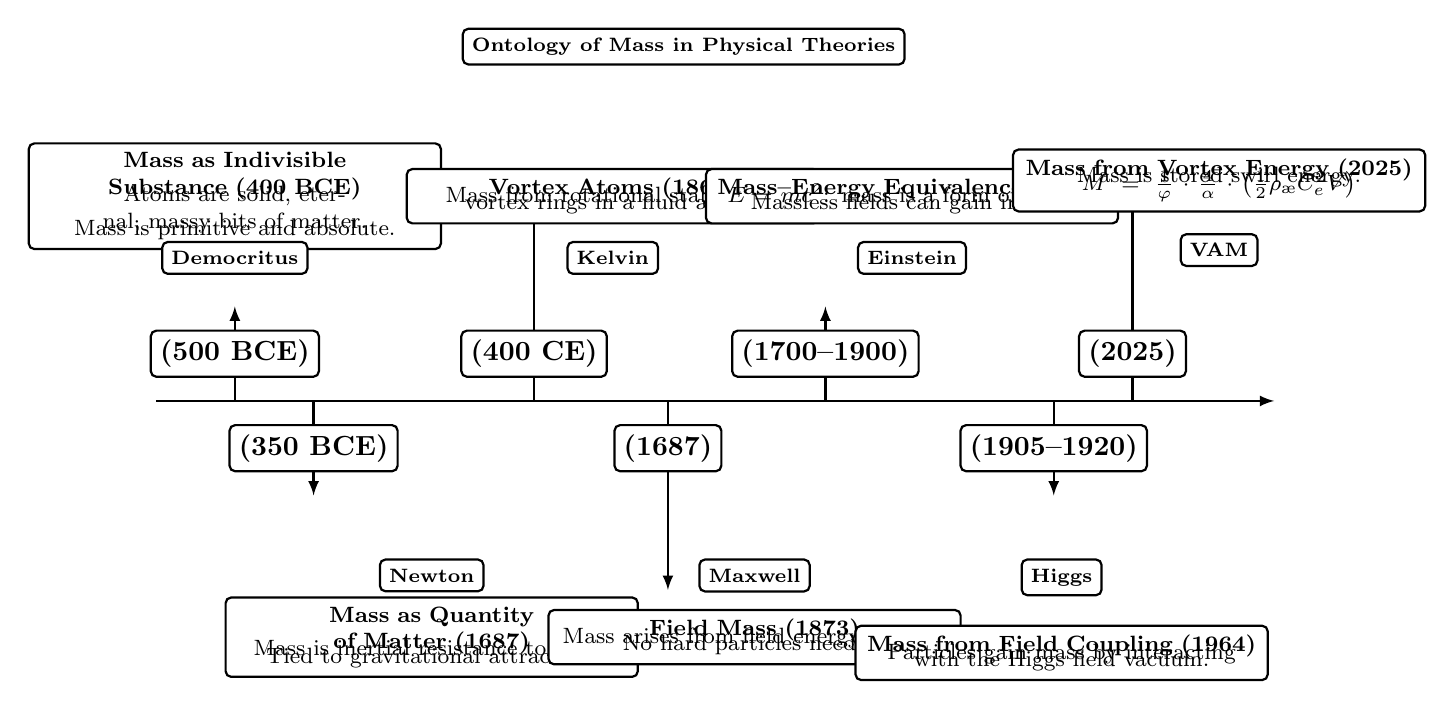
\begin{tikzpicture}[node distance=3.5cm, every node/.style={font=\footnotesize}, >=latex]


% Timeline base
\draw[->, thick] (-1,0) -- (13.2,0);

% Arrows above timeline (short, as requested)
\draw[->, thick] (0,0) -- (0,1.2);       % Pre-Socratics
\draw[->, thick] (3.8,0) -- (3.8,2.5);   % Augustine
\draw[->, thick] (7.5,0) -- (7.5,1.2);   % Einstein
\draw[->, thick] (11.4,0) -- (11.4,3.0); % VAM

% Arrows below timeline (short, as requested)
\draw[->, thick] (1.0,0) -- (1.0,-1.2);     % Plato/Aristotle
\draw[->, thick] (5.5,0) -- (5.5,-2.4);     % Newton
\draw[->, thick] (10.4,0) -- (10.4,-1.2);     % Leibniz/Mach

    %--- Root title cards (above timeline) ---
\node[draw, thick, rounded corners=2pt, fill=white, align=center, font=\bfseries ] at (0, .6)   {(500 BCE)};
\node[draw, thick, rounded corners=2pt, fill=white, align=center, font=\bfseries ] at (3.8, .6) {(400 CE)};
\node[draw, thick, rounded corners=2pt, fill=white, align=center, font=\bfseries ] at (7.5, .6) {(1700--1900)};
\node[draw, thick, rounded corners=2pt, fill=white, align=center, font=\bfseries ] at (11.4, .6){(2025)};

%--- Root title cards (below timeline) ---
\node[draw, thick, rounded corners=2pt, fill=white, align=center, font=\bfseries ] at (1.0,- .6) {(350 BCE)};
\node[draw, thick, rounded corners=2pt, fill=white, align=center, font=\bfseries ] at (5.5,- .6) {(1687)};
\node[draw, thick, rounded corners=2pt, fill=white, align=center, font=\bfseries ] at (10.4,- .6) {(1905--1920)};

% Label
\node[draw, thick, fill=white, rounded corners=2pt, font=\scriptsize] at (5.7,4.5) {\textbf{Ontology of Mass in Physical Theories}};

% Democritus (left)
\node[draw, rounded corners=2pt, thick, align=center, fill=white, text width=5cm] at (0,2.6) {
\textbf{Mass as Indivisible Substance (400 BCE)}  \\[-0.8em]
Atoms are solid, eternal, massy bits of matter.  \\[-0.8em]
Mass is primitive and absolute.
};

\node[above=1.6cm, draw, thick, fill=white, rounded corners=2pt, font=\scriptsize] at (0,0) {\textbf{Democritus}};

% Newton (below)
\node[draw, rounded corners=2pt, thick, align=center, fill=white, text width=5cm] at (2.5,-3.0) {
\textbf{Mass as Quantity of Matter (1687)}  \\[-0.8em]
Mass is inertial resistance to force.  \\[-0.8em]
Tied to gravitational attraction.
};

\node[below=2.0cm, draw, thick, fill=white, rounded corners=2pt, font=\scriptsize] at (2.5,0) {\textbf{Newton}};

% Kelvin (top)
\node[draw, rounded corners=2pt, thick, align=center, fill=white, text width=5cm] at (4.8,2.6) {
\textbf{Vortex Atoms (1867)}  \\[-0.8em]
Mass from rotational stability of  \\[-0.8em]
vortex rings in a fluid æther.
};

\node[above=1.6cm, draw, thick, fill=white, rounded corners=2pt, font=\scriptsize] at (4.8,0) {\textbf{Kelvin}};

% Maxwell (bottom)
\node[draw, rounded corners=2pt, thick, align=center, fill=white, text width=5cm] at (6.6,-3.0) {
\textbf{Field Mass (1873)}  \\[-0.8em]
Mass arises from field energy density.  \\[-0.8em]
No hard particles needed.
};

\node[below=2.0cm, draw, thick, fill=white, rounded corners=2pt, font=\scriptsize] at (6.6,0) {\textbf{Maxwell}};

% Einstein (top)
\node[draw, rounded corners=2pt, thick, align=center, fill=white, text width=5cm] at (8.6,2.6) {
\textbf{Mass–Energy Equivalence (1905)}  \\[-0.8em]
\( E = mc^2 \): mass is a form of energy.  \\[-0.8em]
Massless fields can gain inertia.
};

\node[above=1.6cm, draw, thick, fill=white, rounded corners=2pt, font=\scriptsize] at (8.6,0) {\textbf{Einstein}};

% Higgs (bottom)
\node[draw, rounded corners=2pt, thick, align=center, fill=white, text width=5cm] at (10.5,-3.2) {
\textbf{Mass from Field Coupling (1964)}  \\[-0.8em]
Particles gain mass by interacting  \\[-0.8em]
with the Higgs field vacuum.
};

\node[below=2.0cm, draw, thick, fill=white, rounded corners=2pt, font=\scriptsize] at (10.5,0) {\textbf{Higgs}};

% VAM (top right)
\node[draw, rounded corners=2pt, thick, align=center, fill=white, text width=5cm] at (12.5,2.8) {
\textbf{Mass from Vortex Energy (2025)}  \\[-0.8em]
Mass is stored swirl energy:  \\[-0.8em]
\( M = \frac{1}{\varphi} \cdot \frac{4}{\alpha} \cdot \left( \frac{1}{2} \rho_\text{\ae} C_e^2 V \right) \)
};

\node[above=1.7cm, draw, thick, fill=white, rounded corners=2pt, font=\scriptsize] at (12.5,0) {\textbf{VAM}};

\end{tikzpicture}
\captionof{figure}{Historical evolution of mass ontology: from indivisible substance to field energy and finally to vortex-stored rotational energy in the ætheric continuum of VAM.}
\end{center}

\section{Emergent Lorentz Symmetry from Swirl Fields}
\label{sec:lorentz_recovery}

While VAM posits an absolute æther frame \(\boldsymbol{\mathcal{N}}\), it nonetheless recovers Lorentz symmetry as an emergent approximation for observers embedded within stable vortex structures. This effective symmetry arises from local swirl-induced time dilation, governed by the relation:
\begin{equation}
    d\tau = dt \sqrt{1 - \frac{|\vec{\omega}|^2}{c^2}},
\end{equation}
which mimics the classical Lorentz contraction formula \(dt' = dt \sqrt{1 - v^2/c^2}\) when angular swirl velocity \(|\vec{\omega}|\) is interpreted as a local velocity surrogate.

\resizebox{\textwidth}{!}{%
      \centering
    \scriptsize
        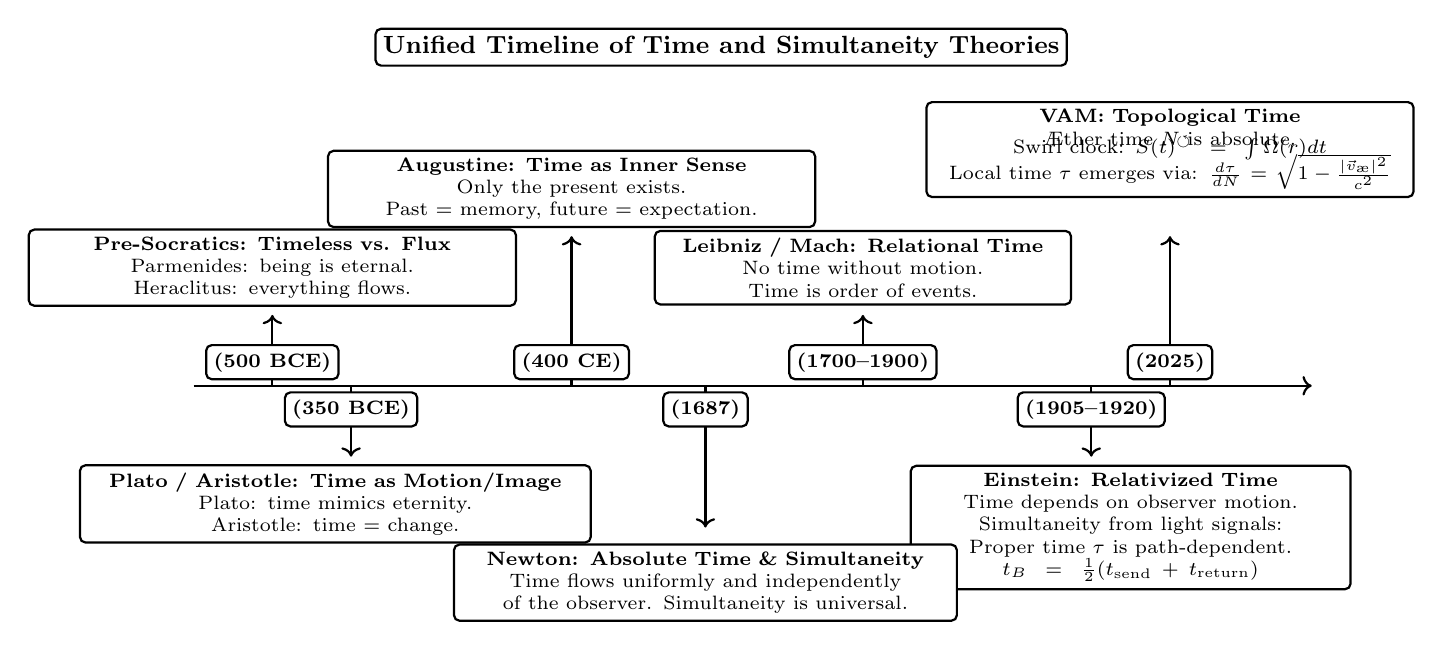
\begin{tikzpicture}
        \scriptsize
        % Timeline base
        \draw[->, thick] (-1,0) -- (13.2,0);

        % Arrows above timeline (short, as requested)
        \draw[->, thick] (0,0) -- (0,0.9);       % Pre-Socratics
        \draw[->, thick] (3.8,0) -- (3.8,1.9);   % Augustine
        \draw[->, thick] (7.5,0) -- (7.5,0.9);   % Einstein
        \draw[->, thick] (11.4,0) -- (11.4,1.9); % VAM

        % Arrows below timeline (short, as requested)
        \draw[->, thick] (1.0,0) -- (1.0,-0.9);     % Plato/Aristotle
        \draw[->, thick] (5.5,0) -- (5.5,-1.8);     % Newton
        \draw[->, thick] (10.4,0) -- (10.4,-0.9);     % Leibniz/Mach

            %--- Root title cards (above timeline) ---
        \node[draw, thick, rounded corners=2pt, fill=white, align=center, font=\bfseries ] at (0, .3)   {(500 BCE)};
        \node[draw, thick, rounded corners=2pt, fill=white, align=center, font=\bfseries ] at (3.8, .3) {(400 CE)};
        \node[draw, thick, rounded corners=2pt, fill=white, align=center, font=\bfseries ] at (7.5, .3) {(1700--1900)};
        \node[draw, thick, rounded corners=2pt, fill=white, align=center, font=\bfseries ] at (11.4, .3){(2025)};

        %--- Root title cards (below timeline) ---
        \node[draw, thick, rounded corners=2pt, fill=white, align=center, font=\bfseries ] at (1.0,- .3) {(350 BCE)};
        \node[draw, thick, rounded corners=2pt, fill=white, align=center, font=\bfseries ] at (5.5,- .3) {(1687)};
        \node[draw, thick, rounded corners=2pt, fill=white, align=center, font=\bfseries ] at (10.4,- .3) {(1905--1920)};

            % Timeline label
        \node[draw, thick, fill=white, rounded corners=2pt, font=\small] at (5.7,4.3) {\textbf{Unified Timeline of Time and Simultaneity Theories}};

        % --- Pre-Socratics ---
        \node[draw, rounded corners=2pt, thick, align=center, fill=white, text width=6cm] at (0,1.5) {
        \textbf{Pre-Socratics: Timeless vs. Flux} \\% [-0.8em]
        Parmenides: being is eternal. \\% [-0.8em]
        Heraclitus: everything flows.
        };

        % --- Augustine ---
        \node[draw, rounded corners=2pt, thick, align=center, fill=white, text width=6cm] at (3.8,2.5) {
        \textbf{Augustine: Time as Inner Sense} \\% [-0.8em]
        Only the present exists. \\% [-0.8em]
        Past = memory, future = expectation.
        };

        % --- Leibniz / Mach ---
        \node[draw, rounded corners=2pt, thick, align=center, fill=white, text width=5.1cm] at (7.5,1.5) {
        \textbf{Leibniz / Mach: Relational Time} \\% [-0.8em]
        No time without motion. \\% [-0.8em]
        Time is order of events.
        };
        % --- VAM (modern) ---
        \node[draw, rounded corners=2pt, thick, align=center, fill=white, text width=6.0cm] at (11.4,3.0) {
        \textbf{VAM: Topological Time} \\% [-0.8em]
        Æther time $N$ is absolute. \\[-0.6em]
        Swirl clock: $S(t)^\circlearrowleft = \int \Omega(r) dt$ \\[-0.4em]
        Local time $\tau$ emerges via: $ \frac{d\tau}{dN} = \sqrt{1 - \frac{|\vec{v}_\text{\ae}|^2}{c^2}}$

        };


        % --- Plato / Aristotle ---
        \node[draw, rounded corners=2pt, thick, align=center, fill=white, text width=6.3cm] at (0.8,-1.5) {
        \textbf{Plato / Aristotle: Time as Motion/Image} \\% [-0.8em]
        Plato: time mimics eternity. \\% [-0.8em]
        Aristotle: time = change.
        };



        % --- Einstein ---
        \node[draw, rounded corners=2pt, thick, align=center, fill=white, text width=5.4cm] at (10.9,-1.8) {
        \textbf{Einstein: Relativized Time} \\% [-0.8em]
        Time depends on observer motion. \\% [-0.8em]
        Simultaneity from light signals: \\% [-0.8em]
        Proper time $\tau$ is path-dependent.\\% [-0.8em]
        $t_B = \frac{1}{2}(t_{\text{send}} + t_{\text{return}})$
        };

        % --- Newton ---
        \node[draw, rounded corners=2pt, thick, align=center, fill=white, text width=6.2cm] at (5.5,-2.5) {
        \textbf{Newton: Absolute Time \& Simultaneity} \\% [-0.8em]
        Time flows uniformly and independently \\% [-0.8em]
        of the observer. Simultaneity is universal.
        };
         \end{tikzpicture}
        \caption{\textbf{Chronology of simultaneity theories across physics and philosophy.} From ancient views of time as change or inner sense, through Newton’s absolute simultaneity and Einstein’s frame-dependent proper time, to VAM’s swirl-based causal layering. The model introduces a physically grounded sequence of time variables culminating in measurable, observer-dependent time ($\tau$) and topological time ($\mathbb{K}$).}\label{fig:history-time-simultaneity}
}


Figure~\ref{fig:history-time-simultaneity} traces the evolving notions of simultaneity and time—from Newton’s absolutes to Einstein’s relativity and the layered temporality of VAM.
Swirl clocks \(S^{\circlearrowleft}_\text{(t)}\) advance slower in regions of high vorticity, reproducing relativistic effects such as time dilation, redshift, and frame dragging. However, unlike in special relativity, these effects are not fundamental symmetries of spacetime but fluid-mechanical consequences of structured vortex motion.

This reinterpretation demotes Lorentz invariance from an a priori principle to a derivative, scale-dependent symmetry—a conclusion supported by multiple derivations across the VAM corpus~\cite{VAM-1, VAM-2, VAM-15}.

\vspace{0.8em}

\noindent\textbf{Ætheric Temporal Sequence:}
\begin{center}
\(\boldsymbol{\mathcal{N}} \to \boldsymbol{\nu_0} \to \boldsymbol{\tau} \to \boldsymbol{S}^{\boldsymbol{\circlearrowleft}}_\text{(t)} \to \boldsymbol{T_v} \to \mathbb{\boldsymbol{K}}\)
\end{center}

    \section{Multimodal Time: The Ætheric Temporal Ontology}\label{sec:multimodal-time:-the-theric-temporal-ontology}
    The Vortex Æther Model (VAM) advances a multimodal conception of time, rooted in the internal and relational dynamics of an incompressible, inviscid æther. Unlike the unidimensional time parameter in standard field theory or the proper time of General Relativity, VAM’s temporal taxonomy encapsulates distinct physical, topological, and informational modes, each with a clear analytical and experimental role. This layered approach not only extends Einstein’s “geometric æther” but also provides a framework for modeling causality, memory, and quantum-classical transitions in a unified manner~\cite{VAM-8, VAM-13, VAM-15}.

\begin{figure}[htb]
    \centering
    \includegraphics[width=0.7\textwidth]{figures/TemporalOntology}
    \caption{
        \textbf{Vortex Phase Spiral of Ætheric Time.} This figure illustrates the sequential emergence of layered temporal modes in the VAM framework, with each governing a distinct aspect of physical law. The progression radiates outward from Aithēr-Time ($\boldsymbol{\mathcal{N}}$), through Now-Point ($\boldsymbol{\nu_0}$), Chronos-Time ($\boldsymbol{\tau}$), Swirl Clock ($\boldsymbol{S}^{\boldsymbol{\circlearrowleft}}_\text{(t)}$), and Vortex Proper Time ($\boldsymbol{T_v}$), to the outermost Kairos Moment ($\mathbb{\boldsymbol{K}}$). These layers form a unified temporal architecture foundational to vortex dynamics~\cite{VAM-8, VAM-13}.
    }

    \label{fig:temporal_ontology}
\end{figure}

The multimodal temporal ontology of VAM is not purely an abstract taxonomy; it possesses a geometric and topological structure, naturally visualized as a multidimensional “spiral” or “fan” in phase space (see Fig.~\ref{fig:temporal_ontology}). This structure parallels phase-space geometries explored in superfluid analog gravity and topological vacua~\cite{volovik2003universe}. Each temporal mode—Aithēr-Time, Now-Point, Chronos-Time, Swirl Clock, Vortex Proper Time, and Kairos Moment—plays an independent yet interconnected role, governing different layers of physical law~\cite{VAM-8, VAM-13}.

\begin{tcolorbox}[
  colback=gray!10,
  colframe=black,
  width=1.0\textwidth,
  sharp corners=southwest,
  boxrule=0.5pt,
  before skip=10pt,
  after skip=10pt,
  title=\textbf{Ætheric Time Modes in the Vortex Æther Model},
  fonttitle=\bfseries,
]
\renewcommand{\arraystretch}{1}
\small
\begin{tabular}{r l l}
  $\boldsymbol{\mathcal{N}}$     & \textbf{Aithēr-Time}         & Absolute causal ordering parameter~\cite{VAM-8, VAM-13} \\
  $\boldsymbol{\nu_0}$           & \textbf{Now-Point}           & Localized intersection with universal present~\cite{VAM-8, VAM-13} \\
  $\boldsymbol{\tau}$            & \textbf{Chronos-Time}        & Measurable time in the æther (subject to dilation)~\cite{VAM-1, VAM-8} \\
  $\boldsymbol{S}^{\boldsymbol{\circlearrowleft}}_\text{(t)}$ & \textbf{Swirl Clock}         & Internal phase memory of a vortex~\cite{VAM-2, VAM-13, VAM-15} \\
  $\boldsymbol{T_v}$             & \textbf{Vortex Proper Time}  & Circulation-based geodesic duration~\cite{VAM-2, VAM-13} \\
  $\mathbb{\boldsymbol{K}}$      & \textbf{Kairos Moment}       & Discrete topological bifurcation event~\cite{VAM-13, VAM-15} \\
\end{tabular}
\end{tcolorbox}

\noindent The interpretation of each mode is as follows:
\begin{itemize}
    \item \textbf{Aithēr-Time ($\boldsymbol{\mathcal{N}}$):} The unobservable but indispensable global time parameter that orders all events causally within the ætheric manifold, serving as the absolute temporal background for physical processes~\cite{VAM-8, VAM-13}.

    \item \textbf{Now-Point ($\boldsymbol{\nu_0}$):} The localized realization of the present, defined by the intersection of the global time field $\boldsymbol{\mathcal{N}}$ with a point in the æther manifold. It establishes the surface of simultaneity and facilitates causal foliation~\cite{VAM-8, VAM-13}.

    \item \textbf{Chronos-Time ($\boldsymbol{\tau}$):} The physically measurable flow of time, experienced within the æther and modulated by local vorticity through swirl-induced time dilation~\cite{VAM-1, VAM-8}:
    \[
        \frac{d\boldsymbol{\tau}}{dt} = \sqrt{1 - \boldsymbol{v_\phi}^2(r)/c^2}
    \]
    where $\boldsymbol{v_\phi}(r)$ is the local tangential velocity of the vortex field.

    \item \textbf{Swirl Clock ($\boldsymbol{S}^{\boldsymbol{\circlearrowleft}}_\text{(t)}$):} The internal phase variable of a vortex structure, tracking angular displacement and serving as a memory function for topological identity and history, drawing from foundational work on helicity conservation and knot topology in vortex dynamics~\cite{knot_theroy_in_fluid}. It is formally given by~\cite{VAM-2, VAM-13}:
    \[
        \boldsymbol{S}^{\boldsymbol{\circlearrowleft}}_\text{(t)} = \int_{0}^{t} \boldsymbol{\Omega}(r(t'))\, dt'
    \]
    with $\boldsymbol{\Omega}(r)$ the local angular velocity.

    \item \textbf{Vortex Proper Time ($\boldsymbol{T_v}$):} The intrinsic circulation-based duration associated with a closed path around a vortex core, defined as~\cite{VAM-2, VAM-13}
    \[
        \boldsymbol{T_v} = \oint \frac{dl}{\boldsymbol{v_\phi}(r)}
    \]
    representing the intrinsic “clock” of a knotted structure.

    \item \textbf{Kairos Moment ($\mathbb{\boldsymbol{K}}$):}
    The discrete event marking a topological transition such as vortex reconnection or bifurcation, producing an irreversible change in vortex identity and introducing discontinuities or non-analyticities in the evolution of $\boldsymbol{T_v}$ or $\boldsymbol{S}^{\boldsymbol{\circlearrowleft}}_\text{(t)}$~\cite{VAM-13, VAM-15}.
\end{itemize}

In the VAM framework, the “Kairos Moment” ($\mathbb{\boldsymbol{K}}$) represents a discrete, topologically induced transition in the evolution of vortex matter—such as a vortex reconnection, bifurcation, or the passage of a gravitational wave. These events break the smooth evolution of then Swirl Clock phase and manifest as quantized phase slips or time jumps. As shown in Fig.~\ref{fig:kairos_moment}, a Kairos event appears as an abrupt change in the Swirl Clock trajectory during a localized temporal window~\cite{buhler2005wave}. Such phenomena are experimentally accessible in analog systems and may be detectable in astrophysical settings as phase anomalies or decoherence events in quantum or classical fields~\cite{VAM-13, VAM-15}. Such temporally localized events have been explored in analogue spacetime geometries where topological phase changes mimic gravitational discontinuities~\cite{barcelo2005}.


\begin{figure}[htb]
    \centering
    \includegraphics[width=0.7\textwidth]{figures/TemporalOntologyKairosMoment}
    \caption{
        \textbf{Swirl Clock Phase Evolution with Kairos Disruption.}
        This figure illustrates the evolution of the Swirl Clock phase, \(\theta(t)\), as a function of Æther Time (\(t
        \)), within the VAM temporal framework. A discrete topological transition—such as vortex reconnection or a passing gravitational wave—introduces a discontinuity in the otherwise smooth phase trajectory.
        The highlighted region, labeled the “Kairos Window,” marks the critical temporal interval where this event occurs. Within this window, the
    vortex structure undergoes an irreversible bifurcation, producing a quantized phase slip or decoherence effect. Such phenomena are defined in VAM as “Kairos Moments” (\(\mathbb{{K}}\)).
        These moments represent a topologically-induced departure from deterministic phase continuity, signaling a transition to a new dynamical regime. Observable manifestations include time “jumps,” phase anomalies, or memory resets within vortex-based systems. Analog experiments in superfluid systems may provide empirical access to these signatures~\cite{VAM-13, VAM-15}.
    }
    \label{fig:kairos_moment}
\end{figure}

This multimodal temporal ontology enables VAM to bridge metaphysical continuity with physically testable vortex dynamics. It underpins several core applications in the extended VAM literature, including models of causality, gravitational time dilation, vortex identity, and swirl-induced phase decoherence~\cite{VAM-1, VAM-2, VAM-8, VAM-13, VAM-15}. For detailed derivations, see~\cite{VAM-2, VAM-8, VAM-13, VAM-15}.

    \section{Connection to the Vortex Æther Model (VAM)}\label{sec:connection_to_VAM}
    The Vortex Æther Model (VAM), developed by O. Iskandarani since 2012, models the æther as an incompressible, non-viscous superfluid~\cite{VAM-8, VAM-13}. Within this framework, vorticity is elevated to a fundamental quantity that governs time dilation, inertial mass, and gravitational interaction~\cite{VAM-2, VAM-10, VAM-13}. Echoing Einstein’s 1920 redefinition of the æther as a physical substratum, VAM treats the æther as a structured, causal medium from which all dynamical behavior emerges~\cite{VAM-8}.

Key structural elements of VAM include:
\begin{itemize}
    \item \textbf{Topological structures} (e.g., knots, trefoils) representing stable particle identities and quantum numbers~\cite{VAM-8, VAM-11, VAM-14},
    \item \textbf{Time dilation} arising from swirl intensity near vortex cores~\cite{VAM-2, VAM-13},
    \item \textbf{A revised system of natural constants}, including $C_e$ (vortex boundary velocity) and $F^{\max}_{\text{\ae}}$ (maximum ætheric stress), defined and operationalized in the topological Lagrangian~\cite{VAM-14}.
\end{itemize}

\subsection*{VAM-Derived Expression for $\boldsymbol{G}$}

One of the notable results in VAM is a derivation of the gravitational constant in terms of ætheric and topological parameters~\cite{VAM-2, VAM-13, VAM-14}. Rewriting the expression in dimensionally transparent form:

\begin{equation}
    G_\text{swirl} = \frac{C_e}{2 F^{\max}_{\text{\ae}}} \cdot \left( \frac{c^5 t_p^2}{r_c^2} \right)
\end{equation}

\noindent where:
\begin{itemize}
    \item $C_e$: swirl velocity at the vortex boundary (m/s),
    \item $F^{\max}_{\text{\ae}}$: maximum force the æther can sustain before bifurcation (N),
    \item $t_p$: Planck time $ \left(\sqrt{\hbar G / c^5}\right) $,
    \item $r_c$: core radius of the vortex structure (m),
    \item $c$: speed of light in vacuum (m/s).
\end{itemize}

This formulation emerges from the Swirl Clock formalism and connects gravity to rotational energy density under conservation of circulation~\cite{VAM-2, VAM-13}. It expresses $G$ not as a fundamental input constant, but as a derived quantity arising from the interplay of topological scale $r_c$, rotational dynamics $C_e$, and ætheric tension $F^{\max}_{\text{\ae}}$. This reinforces the view that gravitation is a residual effect of conserved vorticity in a compressible ætheric medium.

VAM further incorporates circulation quantization, helicity conservation, and pressure-mediated interactions to model the exchange between knotted structures and their surrounding swirl fields~\cite{VAM-8, VAM-11, VAM-14}. This general framework aligns with Einstein’s late attempt at a unified field theory—now realized through the mathematics of topological fluid dynamics.

The model's predictions are experimentally approachable through analog systems such as rotating superfluid vortices, BEC interference patterns, and refractive index shifts under swirl acceleration~\cite{VAM-2, VAM-13}. These offer testable pathways for validating the core dynamics proposed by VAM.

\vspace{1em}

    \section{Historical Continuity and Outlook}\label{sec:historical-continuity-and-outlook}
    A careful reexamination of Einstein's later writings reveals that he:
\begin{itemize}
    \item Did \emph{not} reject the æther outright, but \emph{redefined} it as a field-carrying substrate~\cite{einstein1920aether},
    \item Sought a \textbf{continuous medium} bearing the properties of spacetime without requiring mechanical motion,
    \item And ultimately pursued a \textbf{unified field theory}—one that VAM now echoes through the interplay of gravity, time perception, and vorticity~\cite{VAM-8, VAM-14}.
\end{itemize}

Einstein recognized that space could not be entirely void—it had to possess structural, energetic, and causal qualities. In this context, the Vortex Æther Model is not a speculative throwback, but a mathematically grounded continuation of Einstein's vision. It operationalizes this active structure via conserved vortex fields, topological knot invariants, and energy-sustaining boundary flows~\cite{VAM-8, VAM-11, VAM-14}.
This approach directly addresses critiques that modern theoretical physics has strayed from empirical accountability in favor of formal aestheticism~\cite{hossenfelder2018lost}.


While other contemporary models—such as emergent gravity and superfluid vacuum theory—have gestured toward similar foundations, VAM distinguishes itself by offering an explicitly solvable, hydrodynamically derived, and testable framework~\cite{VAM-8, VAM-14, VAM-15}. It bridges general relativity, thermodynamics, and quantum field heuristics without requiring discrete particles or quantized spacetime.

Kelvin's concern regarding topological degeneracy is addressed in Appendix~\ref{appendix:kelvin}.


\section*{Conclusion and Forward Outlook: Æther Reclaimed}

Modern theoretical physics is gradually converging on insights once considered obsolete—not because the underlying concepts were invalid, but because earlier mathematical and experimental tools lacked the necessary precision. Einstein’s late-career perspective on the æther anticipated this renaissance: a vision of space as a continuous, energetic, and causally structured medium. The Vortex Æther Model (VAM) builds directly on this foundation, advancing it into a unified, predictive, and testable framework~\cite{VAM-8, VAM-13, VAM-14}.

Here, vorticity and topological structure supplant the classical notion of curvature, and time itself emerges as a hierarchy of circulation and phase—fully realized in the multimodal temporal ontology~\cite{VAM-13, VAM-15}. The æther, once dismissed, returns in a new form: not as a mechanical ether, but as a quantized, causal, and observable substrate underlying all known phenomena—from gravitation and particle masses to quantum measurement and cosmological evolution~\cite{VAM-8, VAM-11, VAM-15, VAM-17.1}.


VAM does not merely offer a philosophical bridge to Einstein’s “unified field” dream, but delivers a rigorous technical foundation and explicit predictions that now invite empirical validation. With advancing experiments in superfluid analogues, quantum vortex interferometry, and photonic swirl, the opportunity to test, refine, or falsify these ideas moves within experimental reach~\cite{VAM-2, VAM-13, VAM-15}.

It is time to move beyond the view of Einstein as the man who abolished the æther, and instead to recognize him as the thinker who quietly reframed it—preparing the ground for its scientific rebirth. In that spirit, the Vortex Æther Model is not a closure, but an opening: a dynamic, empirically accessible, and mathematically coherent path forward in the ongoing quest for a unified physical theory.

Several testable predictions arise from the VAM framework. Swirl-induced time dilation may be observed through analog vortex systems in rotating superfluid helium or Bose–Einstein condensates. Vortex reconnection events can be simulated in quantum fluid platforms to probe discontinuities in Swirl Clock phase (Kairos transitions). Moreover, anomalous frame-dragging profiles predicted by VAM could, in principle, be detected in precision interferometry experiments. Future work will expand the observable phenomenology of the model, bridging theory with laboratory and astrophysical data.


\subsection*{Future Directions and Experimental Signatures}

The path forward for the Vortex Æther Model is both theoretically rich and experimentally accessible. On the theoretical front, continued development will further refine the topological classification of particle states~\cite{VAM-11, VAM-14}, explore fractal swirl dynamics at both quantum and cosmological scales~\cite{VAM-12, VAM-9}, and formalize the mechanisms by which gravitation and quantum phenomena emerge from circulation and helicity conservation~\cite{VAM-13, VAM-15}.

Empirically, the VAM framework provides several concrete predictions and signatures amenable to near-future tests:
\begin{itemize}
    \item \textbf{Time dilation and frame-dragging effects} in laboratory superfluids, Bose–Einstein condensates, and photonic vortex lattices~\cite{VAM-2, VAM-13};
    \item \textbf{Swirl clock phase slips and Kairos events} observable as quantized phase jumps or decoherence in quantum vortex interferometry~\cite{VAM-15};
    \item \textbf{Anomalous redshift, light bending, and perihelion precession} in astrophysical observations that deviate from standard General Relativity in high-vorticity or topologically complex environments~\cite{VAM-10};
    \item \textbf{Spectral and mass predictions} for leptons, baryons, and their excited states, determined by knot topology and quantized circulation~\cite{VAM-11, VAM-14};
    \item \textbf{Novel cosmological signatures} arising from large-scale swirl structure and the fractal dynamics of the æther, potentially visible in galaxy rotation curves and the cosmic microwave background~\cite{VAM-9, VAM-12}.
\end{itemize}

By combining theoretical coherence with falsifiable experimental predictions, the Vortex Æther Model opens a concrete research agenda for unifying gravitation, quantum mechanics, and cosmology. As the boundaries of precision measurement and analog simulation continue to expand, VAM stands poised to guide and interpret the next wave of discoveries at the intersection of topology, fluid dynamics, and fundamental physics. Future work will also integrate recent results on the photon as a quantized vortex excitation~\cite{VAM-17.1} into the broader particle taxonomy, connecting topological charge to quantum numbers.


    \appendix

        \section*{Appendix I: Helmholtz and the Foundations of Vortex Physics}
        \addcontentsline{toc}{section}{Appendix I: Helmholtz on Vorticity}
            \label{appendix:helmholtz}
                Hermann von Helmholtz’s 1858 paper \textit{“On the Integrals of the Hydrodynamic Equations Corresponding to Vortex Motion”}~\cite{helmholtz1858vortices} marks the formal beginning of vortex theory in physics. His theorems define the behavior of vorticity in an ideal, incompressible fluid—concepts foundational to the Vortex Æther Model (VAM).

    \subsection*{1. Vorticity is conserved along fluid lines}
    \begin{quote}
    \textit{“Each portion of a vortex filament remains connected to the same fluid elements throughout the motion.”}
    \end{quote}

    \textbf{VAM Mapping:} This becomes the core of VAM’s knot stability. Swirl identity is maintained via conserved helicity and circulation:
    \[
    \frac{d\Gamma}{dt} = 0, \quad \Gamma = \oint_{\mathcal{C}} \vec{v} \cdot d\vec{\ell}
    \]

    \subsection*{2. Vortex lines cannot end in a fluid — they form closed loops or extend to boundaries}
    \begin{quote}
    \textit{“The extremities of a vortex line cannot exist within the fluid; they must lie at the boundaries or form closed curves.”}
    \end{quote}

    \textbf{VAM Mapping:} Explains the closed-loop structure of particle-knot analogues in VAM. Vortices are topologically confined:
    \[
    \nabla \cdot \vec{\omega} = 0
    \]

    \subsection*{3. Circulation is invariant under ideal flow}
    \begin{quote}
    \textit{“The circulation around a closed curve moving with the fluid remains constant.”}
    \end{quote}

    \textbf{VAM Mapping:} VAM uses this to define internal clocks, mass, and swirl energy. This law becomes the origin of the time dilation formula:
    \[
    S(t) = \int \omega(t) \, dt, \quad T_v \sim \Gamma^{-1}
    \]

    \subsection*{Historical Legacy}

    Helmholtz's influence extended deeply into Kelvin’s vortex atom theory, Maxwell’s mechanical æther models, and later Einsteinian field theory. Today, in the Vortex Æther Model, his principles live on as conservation laws that define both structure and evolution of the physical vacuum.

    \begin{quote}
    \textit{“If matter is vortex, then Helmholtz is its first architect.”}
    \end{quote}
   \hfill — O. Iskandarani


        \section*{Appendix II: Lord Kelvin and the Knot-Æther Critique}
        \addcontentsline{toc}{section}{Appendix II: Lord Kelvin}
            \label{appendix:kelvin}
               In the late 19th century, William Thomson (Lord Kelvin) proposed that atoms might be stable vortex knots in an invisible æther — a topological interpretation of matter. Yet he himself raised the most pointed critique:

   \begin{quote}
   \("\) I am afraid of the smoke and complication, of all the varieties of knots and links, if they are to explain the variety of elements.\("\)
   \end{quote}
\hfill  — Lord Kelvin, 1890

   Kelvin feared that the near-infinite number of possible knots and links in three-dimensional space would not correspond to the relatively small number of stable chemical elements~\cite{thomson1890knots, tait1877knots}. Without a natural principle of selection, the theory risked degeneracy: the proliferation of mathematically possible but physically irrelevant structures.

   \subsection*{Historical Context}

   In the second half of the 19th century, the vortex atom theory was developed, primarily by William Thomson (Lord Kelvin) and Peter Guthrie Tait~\cite{thomson1890knots, tait1877knots}. In this framework, atoms were envisioned as stable knots or vortex rings in an ideal, invisible fluid — the so-called luminiferous æther. The idea was that both the discrete nature of atomic species and their remarkable stability could be explained through topological invariants from knot theory.

   Helmholtz's 1858 paper introduced the conservation of vorticity in ideal fluids, laying the mathematical foundation upon which Kelvin and Tait constructed the vortex atom theory~\cite{helmholtz1858vortices}. This conservation principle is central to both classical vortex stability and the topological persistence employed in VAM.

   Kelvin's model was deeply influenced by the work of Helmholtz (1858) on vortex conservation in ideal fluids. He imagined that different types of knotted or linked vortices might correspond to different elements.

   \subsection*{Kelvin's Principal Objection}

   Despite its elegance, Kelvin identified a critical flaw:

   \begin{quote}
   \("\) I am afraid of the smoke and complication, of all the varieties of knots and links, if they are to explain the variety of elements.\("\)
   \end{quote}\\
    \hfill — William Thomson (Lord Kelvin), Baltimore Lectures, 1890\\
   The mathematical space of knots is vast, and Kelvin recognized the absence of a physical filter. He was acutely aware that the theory, though geometrically rich, lacked a way to explain *why only some knots should be stable atoms*. It had no built-in energetic, dynamic, or entropic selection rule.

   \subsection*{Experimental Shortcomings}

   Kelvin also noted the absence of empirical correspondence between specific knot types and actual elements. Without experimental access to the supposed vortex knots — their formation, stability, or interaction — the theory remained speculative.

   Nonetheless, the idea lived on, inspiring both topological mathematics and future models of discrete matter arising from continuous media.

   \subsection*{Comparison to the Modern Particle Zoo}

   Kelvin's critique is echoed in modern particle physics. The Standard Model contains a large number of particles, generations, couplings, and constants — many set only by experimental input, not derivable from deeper principles.

   \begin{quote}
   \textit{\("\) I am afraid I must end by saying that the difficulties are so great in the way of forming anything like a comprehensive theory, that we cannot even imagine a finger-post pointing to a way that leads us towards the explanation.} \\
   \textit{But this time next year — this time ten years — this time one hundred years — I cannot doubt but that these things which now seem to us so mysterious will be no mysteries at all. The scales will fall from our eyes. We shall learn to look on things in a different way — when that which is now a difficulty will be the only common-sense and intelligible way of looking at the subject.\("\)}
   \end{quote}
   \hfill — *Lord Kelvin, circa 1889*

   The degeneracy Kelvin foresaw reappears: a theory with many admissible but unexplained types of particles. The need for a *selection mechanism* remains urgent.

   \subsection*{The VAM Response}

   The Vortex Æther Model (VAM) revives the topological atom intuition but answers Kelvin's critique with concrete physical principles:

   \begin{itemize}
     \item Thermodynamic constraints (via Clausius entropy) limit allowable knot growth~\cite{clausius1865entropy}.
     \item Quantized circulation excludes unstable, high-energy configurations.
     \item Absolute vorticity conservation enforces topological stability.
     \item Vortex reconnection thresholds act as evolutionary boundaries.
   \end{itemize}

   As a result, VAM predicts only a finite, physically meaningful spectrum of topological matter structures — in line with observed baryons and leptons.

   \subsection*{Concluding Reflection}

   Kelvin's objection was not to knots themselves, but to their uncontrolled proliferation. VAM reclaims his vision, but grounds it in hydrodynamic logic, energy bounds, and field evolution:

   \begin{quote}
    \("\) Knots without constraints become chaos. Knots with physics become atoms.\("\)
   \end{quote}
  \hfill — O. Iskandarani


        \section*{Appendix III: James Clerk Maxwell on the Æther and the Vortex Atom Theory}
        \addcontentsline{toc}{section}{Appendix III: James Clerk Maxwell on the Æther and the Vortex Atom Theory}
            \label{appendix:maxwell}
            \input{A3_Maxwell}

        \section*{Appendix IV: Einstein on the Æther — Translated Quotes and VAM Equivalents}
        \addcontentsline{toc}{section}{Appendix IV: Einstein on the Æther}
            \label{appendix:einstein}
            This appendix collects and annotates key statements made by Albert Einstein about the æther, focusing especially on how these statements align or contrast with the structure and assumptions of the Vortex Æther Model (VAM). Where possible, original German excerpts are included, with English translations and a mapping to VAM concepts or equations.

\subsection*{1. \grqq Der Raum ohne Äther ist undenkbar...\textquotedblright}
\textbf{Original (1920 Leiden Lecture):} \\
\("\)Nach der allgemeinen Relativitätstheorie ist der Raum mit physikalischen Eigenschaften begabt; in diesem Sinne existiert also ein Äther. Gemäß der allgemeinen Relativitätstheorie ist ein Raum ohne Äther undenkbar.\("\)

\textbf{Translation:} \\
\("\)According to the general theory of relativity, space is endowed with physical qualities; in this sense, therefore, there exists an æther. According to the general theory of relativity, space without æther is unthinkable.\("\)

\textbf{VAM Mapping:} \\
This matches VAM's foundational postulate that the æther is a structured, non-viscous, incompressible medium with internal physical dynamics. The VAM equivalent is the existence of a vorticity-carrying background field \( \vec{\omega}(\vec{r}, t) \), subject to conservation laws and boundary conditions.

\[
\nabla \cdot \vec{v} = 0, \quad \nabla \cdot \vec{\omega} = 0, \quad \partial_t \vec{\omega} + (\vec{v} \cdot \nabla) \vec{\omega} = (\vec{\omega} \cdot \nabla) \vec{v}
\]

\subsection*{2. \grqq Es scheint, als sei die Einführung eines Äthers überflüssig...\textquotedblright}
\textbf{Original (1905, SR paper):} \\
\("\)Es scheint, als sei die Einführung eines Äthers überflüssig, insofern die Lichtausbreitung durch Maxwell'sche Gleichungen in leerem Raum ausreichend beschrieben werden kann.\("\)

\textbf{Translation:} \\
\("\)It seems that the introduction of an æther is superfluous, insofar as the propagation of light can be described adequately by Maxwell's equations in vacuum.\("\)

\textbf{VAM Mapping:} \\
Einstein's 1905 view was contextually specific to the Maxwellian field theory. VAM expands this to a \emph{sub-Maxwellian} fluid substrate: the fields emerge from vortex dynamics.

VAM introduces: \\
\( \vec{E} = -\nabla \Phi - \partial_t \vec{A}, \quad \vec{B} = \nabla \times \vec{A} \) as secondary fields derived from swirl-based potentials in the æther.

\subsection*{3. \grqq Der Äther darf nicht als ein Medium mit mechanischen Eigenschaften gedacht werden...\textquotedblright}
\textbf{Original (1920):} \\
\("\)Der Äther darf nicht als ein Medium mit mechanischen Eigenschaften gedacht werden, wie es die alten Ätherkonzepte vorschlugen. Er besitzt keine Bewegungen, wie z.B. Geschwindigkeit.\("\)

\textbf{Translation:} \\
\("\)The æther must not be thought of as a medium with mechanical properties, as the old concepts of æther suggested. It has no motion in the usual sense, like velocity.\("\)

\textbf{VAM Mapping:} \\
In VAM, the æther has \emph{field-like behavior}, not particulate or elastic-body behavior. The \grqq no absolute velocity\textquotedblright principle is respected via invariance under global coordinate transformation, but local rotational states \( \vec{\omega} \neq 0 \) define structure. Time dilation depends on vorticity~\cite{VAM-2}:

\[
\frac{d\tau}{dt} = \sqrt{1 - \frac{C_e^2}{c^2} e^{-r/r_c}}
\]

\subsection*{4. \grqq Das Gravitationsfeld selbst kann als ein Zustand dieses Äthers angesehen werden.\textquotedblright}
\textbf{Original (1920):} \\
\("\)Das Gravitationsfeld selbst kann als ein Zustand dieses Äthers angesehen werden.\("\)

\textbf{Translation:} \\
\("\)The gravitational field itself can be regarded as a state of this æther.\("\)

\textbf{VAM Mapping:} \\
This is directly analogous to the VAM interpretation of gravity: not as spacetime curvature, but as an emergent effect of vorticity-induced pressure gradients:

\[
\nabla P = \rho_\text{\ae} \vec{a} = -\frac{1}{2} \rho_\text{\ae} \nabla |\vec{\omega}|^2
\]

\subsection*{5. \grqq Die Zeit ist in einem Gravitationsfeld anders definiert...\textquotedblright}
\textbf{Original (1916, Grundlagen der ART):} \\
\("\)Die Zeit ist in einem Gravitationsfeld anders definiert als in der Abwesenheit desselben; die Zeitdifferenz hängt von der Lage im Feld ab.\("\)

\textbf{Translation:} \\
\("\)Time is defined differently in a gravitational field than in its absence; the time differential depends on the position within the field.\("\)

\textbf{VAM Mapping:} \\
This statement supports VAM's approach of \emph{local time dilation} derived from rotational energy density and vorticity:

\[
\frac{d\tau}{dt} = \sqrt{1 - \frac{1}{U_\text{max}} U_{\text{vortex}}} = \sqrt{1 - \frac{1}{2U_\text{max}} \rho_\text{\ae} |\vec{\omega}|^2}
\]

\bigskip
\textit{ \("\) Einstein did not eliminate the æther. He redefined it. VAM takes the next step. \("\)}\\
\hfill — O. Iskandarani\\

        \section*{Appendix V: VAM Resolution of Einstein’s Final Æther Paradox}
        \addcontentsline{toc}{section}{Appendix V: VAM and the Final Æther Paradox}
            \label{appendix:final-aether}
            
\vspace{1em}
\subsubsection*{Einstein’s Final Æther Statement (1920)}
\begin{quote}
\small
“Space without æther is unthinkable; for in such space there not only would be no propagation of light, but also no possibility of existence for standards of space and time (measuring-rods and clocks), nor therefore any space-time intervals in the physical sense. But this æther may not be thought of as endowed with the quality characteristic of ponderable media, as consisting of parts which may be tracked through time. The idea of motion may not be applied to it.”
\end{quote}

\noindent\textbf{The paradox:}  Einstein’s statement crystallizes his ultimate æther paradox: space must be endowed with physical qualities (an æther), yet the æther must possess \emph{no trackable motion}, no mechanical parts, and no temporally evolving components. The æther is thus essential but static—a silent scaffolding for relativistic structure.

\medskip

\subsubsection*{VAM Resolution: Internal Motion Without Bulk Translation}
The Vortex Æther Model (VAM) resolves this paradox by distinguishing between bulk translational motion and internal rotational structure:

\begin{itemize}
    \item The æther is \textbf{incompressible and inviscid}, preserving the continuum assumptions of fluid dynamics.
    \item It is \textbf{globally at rest} (\( \vec{v}_{\text{bulk}} = 0 \)), with no net velocity relative to absolute space.
    \item It is \textbf{locally dynamic}, supporting conserved vorticity and phase evolution:
    \[
        \boldsymbol{\omega} = \nabla \times \vec{v}, \qquad
        \vec{v}(r) = \frac{C_e}{r} e^{-r/r_c} \, \hat{\theta}
    \]
    \item It is \textbf{temporally causal}, with internal memory encoded in the swirl clock phase:
    \[
        \boldsymbol{S}(t) = \int \Omega(r) \, dt = \int \frac{C_e}{r_c} e^{-r/r_c} dt
    \]
\end{itemize}
No “parts” are tracked spatially, but topological invariants (vortex knots, helicity, linking number) serve as memory carriers—fulfilling Einstein’s requirements without violating his restrictions.


\medskip

\subsubsection*{Clocks and Rods from Swirl Geometry}
Einstein argued that standards of space and time (measuring rods, clocks) require a nontrivial substrate. In VAM:
\begin{itemize}
    \item Both are emergent from local swirl structures. A “particle” is a \textbf{knotted vortex loop} with angular frequency \( \Omega \), circulation \( \Gamma \), and internal energy:
    \[
        U_{\text{vortex}} = \frac{1}{2} \rho_\text{\ae}^{(\text{energy})} |\boldsymbol{\omega}|^2
    \]
    \item Time dilation near such a structure follows:
    \[
        \frac{d\tau}{dt} = \sqrt{1 - \frac{U_{\text{vortex}}}{U_{\text{max}}}} = \sqrt{1 - \frac{1}{2U_{\text{max}}} \rho_\text{\ae}^{(\text{energy})} |\boldsymbol{\omega}|^2}
    \]
    \item Thus, “clocks” and “rods” are \emph{manifestations of local energetics and topology}, not primitive objects.
\end{itemize}

\medskip

\subsubsection*{Reinterpreting “No Trackable Parts”}
Einstein forbade tracking “parts” of the æther through time. In VAM:
\begin{itemize}
    \item Fluid elements are not tracked by position;
    \item Instead, \textbf{vortex filaments} and their topological invariants (\( \ell \), \( H \), \( K \)) encode causal evolution and system memory;
    \item These are not particulate—they are \emph{topological excitations}, reconciling Einstein’s view with a physically rich substrate.
\end{itemize}

\medskip

\subsubsection*{Conclusion: From Silent Substrate to Structured Swirl}
Where Einstein’s æther was a silent backdrop enabling relativity, VAM’s æther is an \emph{active but non-translating medium} whose internal structure encodes mass, time, inertia, and gravity.
\vspace{0.5em}


\begin{quote}
\textit{“Einstein stripped the æther of velocity to preserve symmetry. VAM restores internal motion to recover substance.”}
\begin{flushright}
— O. Iskandarani
\end{flushright}
\end{quote}

        \section{Appendix VI: Simultaneity — From Light Pulses to Vortex Clocks}
        \addcontentsline{toc}{section}{Appendix VI: Simultaneity — From Light Pulses to Vortex Clocks}
            \label{appendix:Simultaneity}
                In Einstein’s theory, time is defined operationally through the arrival and departure of light signals. Simultaneity is not absolute, but constructed by coordinating photon trajectories between clocks. This makes time a relational concept—dependent on the motion of observers and the invariance of light speed.

    \begin{table}[h!]
        \centering
        \begin{tabular}{|c|c|c|c|}
            \hline
            \textbf{Theory} & \textbf{Time} & \textbf{Simultaneity} & \textbf{Defined By} \\
            \hline
            Newton & Absolute & Universal & External flow of time \\
            Einstein (SR/GR) & Relative & Frame-dependent & Light signal coordination \\
            VAM & Layered (N, $\tau$, $S(t)$) & Phase-coherent & Vortex swirl phase $\Omega(r)$ \\
            \hline
        \end{tabular}
        \caption{Comparison of time and simultaneity in Newtonian, Einsteinian, and VAM frameworks.}
    \end{table}

    In contrast, the Vortex Æther Model grounds time in the internal dynamics of the medium itself. Absolute æther time \( N \) flows uniformly, while local time \( \tau \) and swirl clock time \( S(t) \) emerge from the rotational energy and helicity of vortex structures. Simultaneity is no longer a matter of synchronization via photons—it is encoded in the shared phase coherence of knotted circulation. In this sense, VAM replaces relativistic light-clock simultaneity with a topologically grounded, energetically conserved temporal ontology.



\resizebox{\textwidth}{!}{%
      \centering
    \scriptsize
        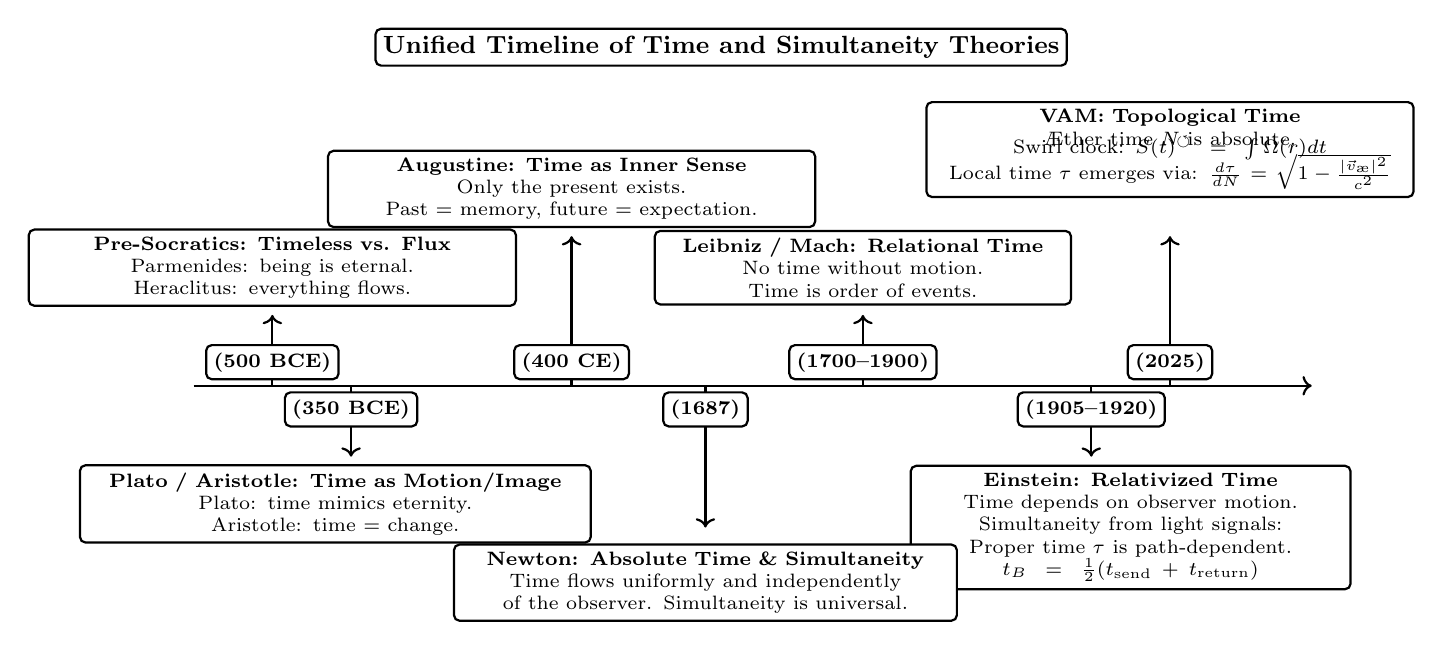
\begin{tikzpicture}
        \scriptsize
        % Timeline base
        \draw[->, thick] (-1,0) -- (13.2,0);

        % Arrows above timeline (short, as requested)
        \draw[->, thick] (0,0) -- (0,0.9);       % Pre-Socratics
        \draw[->, thick] (3.8,0) -- (3.8,1.9);   % Augustine
        \draw[->, thick] (7.5,0) -- (7.5,0.9);   % Einstein
        \draw[->, thick] (11.4,0) -- (11.4,1.9); % VAM

        % Arrows below timeline (short, as requested)
        \draw[->, thick] (1.0,0) -- (1.0,-0.9);     % Plato/Aristotle
        \draw[->, thick] (5.5,0) -- (5.5,-1.8);     % Newton
        \draw[->, thick] (10.4,0) -- (10.4,-0.9);     % Leibniz/Mach

            %--- Root title cards (above timeline) ---
        \node[draw, thick, rounded corners=2pt, fill=white, align=center, font=\bfseries ] at (0, .3)   {(500 BCE)};
        \node[draw, thick, rounded corners=2pt, fill=white, align=center, font=\bfseries ] at (3.8, .3) {(400 CE)};
        \node[draw, thick, rounded corners=2pt, fill=white, align=center, font=\bfseries ] at (7.5, .3) {(1700--1900)};
        \node[draw, thick, rounded corners=2pt, fill=white, align=center, font=\bfseries ] at (11.4, .3){(2025)};

        %--- Root title cards (below timeline) ---
        \node[draw, thick, rounded corners=2pt, fill=white, align=center, font=\bfseries ] at (1.0,- .3) {(350 BCE)};
        \node[draw, thick, rounded corners=2pt, fill=white, align=center, font=\bfseries ] at (5.5,- .3) {(1687)};
        \node[draw, thick, rounded corners=2pt, fill=white, align=center, font=\bfseries ] at (10.4,- .3) {(1905--1920)};

            % Timeline label
        \node[draw, thick, fill=white, rounded corners=2pt, font=\small] at (5.7,4.3) {\textbf{Unified Timeline of Time and Simultaneity Theories}};

        % --- Pre-Socratics ---
        \node[draw, rounded corners=2pt, thick, align=center, fill=white, text width=6cm] at (0,1.5) {
        \textbf{Pre-Socratics: Timeless vs. Flux} \\% [-0.8em]
        Parmenides: being is eternal. \\% [-0.8em]
        Heraclitus: everything flows.
        };

        % --- Augustine ---
        \node[draw, rounded corners=2pt, thick, align=center, fill=white, text width=6cm] at (3.8,2.5) {
        \textbf{Augustine: Time as Inner Sense} \\% [-0.8em]
        Only the present exists. \\% [-0.8em]
        Past = memory, future = expectation.
        };

        % --- Leibniz / Mach ---
        \node[draw, rounded corners=2pt, thick, align=center, fill=white, text width=5.1cm] at (7.5,1.5) {
        \textbf{Leibniz / Mach: Relational Time} \\% [-0.8em]
        No time without motion. \\% [-0.8em]
        Time is order of events.
        };
        % --- VAM (modern) ---
        \node[draw, rounded corners=2pt, thick, align=center, fill=white, text width=6.0cm] at (11.4,3.0) {
        \textbf{VAM: Topological Time} \\% [-0.8em]
        Æther time $N$ is absolute. \\[-0.6em]
        Swirl clock: $S(t)^\circlearrowleft = \int \Omega(r) dt$ \\[-0.4em]
        Local time $\tau$ emerges via: $ \frac{d\tau}{dN} = \sqrt{1 - \frac{|\vec{v}_\text{\ae}|^2}{c^2}}$

        };


        % --- Plato / Aristotle ---
        \node[draw, rounded corners=2pt, thick, align=center, fill=white, text width=6.3cm] at (0.8,-1.5) {
        \textbf{Plato / Aristotle: Time as Motion/Image} \\% [-0.8em]
        Plato: time mimics eternity. \\% [-0.8em]
        Aristotle: time = change.
        };



        % --- Einstein ---
        \node[draw, rounded corners=2pt, thick, align=center, fill=white, text width=5.4cm] at (10.9,-1.8) {
        \textbf{Einstein: Relativized Time} \\% [-0.8em]
        Time depends on observer motion. \\% [-0.8em]
        Simultaneity from light signals: \\% [-0.8em]
        Proper time $\tau$ is path-dependent.\\% [-0.8em]
        $t_B = \frac{1}{2}(t_{\text{send}} + t_{\text{return}})$
        };

        % --- Newton ---
        \node[draw, rounded corners=2pt, thick, align=center, fill=white, text width=6.2cm] at (5.5,-2.5) {
        \textbf{Newton: Absolute Time \& Simultaneity} \\% [-0.8em]
        Time flows uniformly and independently \\% [-0.8em]
        of the observer. Simultaneity is universal.
        };
         \end{tikzpicture}
        \caption{\textbf{Chronology of simultaneity theories across physics and philosophy.} From ancient views of time as change or inner sense, through Newton’s absolute simultaneity and Einstein’s frame-dependent proper time, to VAM’s swirl-based causal layering. The model introduces a physically grounded sequence of time variables culminating in measurable, observer-dependent time ($\tau$) and topological time ($\mathbb{K}$).}\label{fig:history-time-simultaneity}
}

\begin{center}
\footnotesize
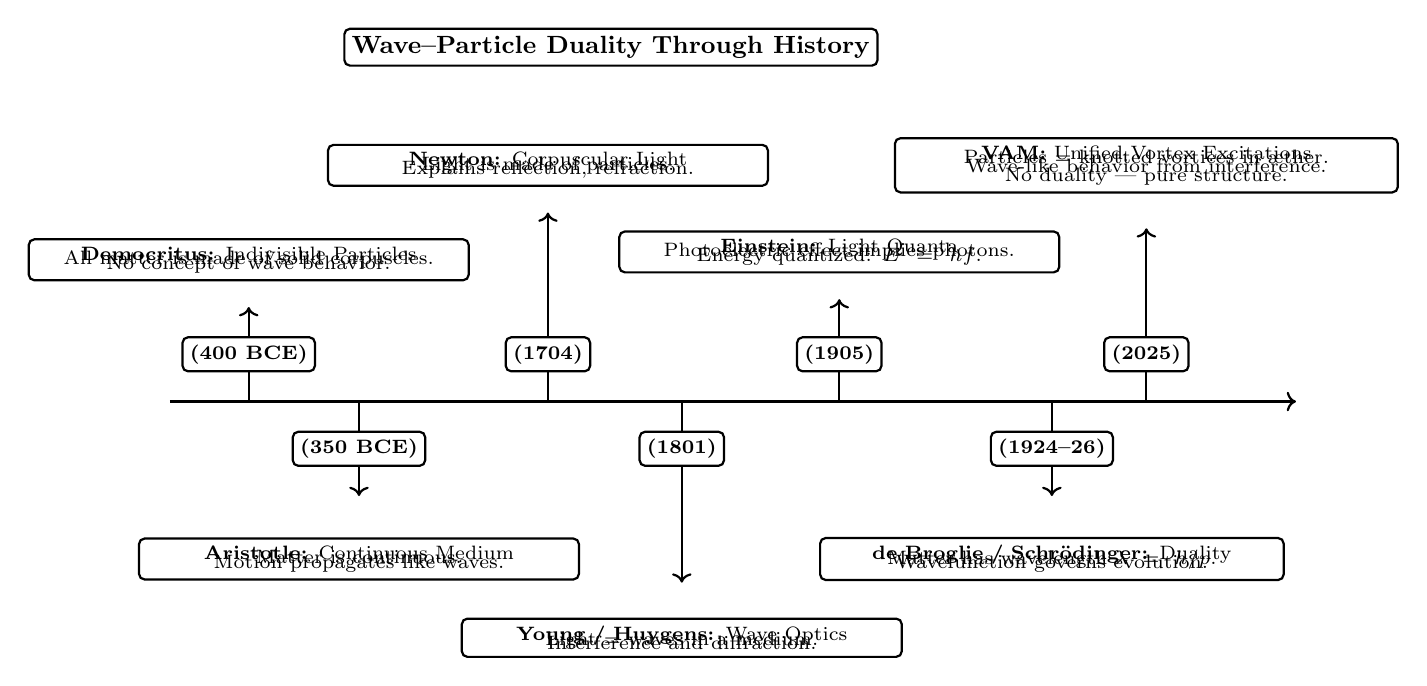
\begin{tikzpicture}
\scriptsize

% Timeline base
\draw[->, thick] (-1,0) -- (13.3,0);

% Arrows above timeline
\draw[->, thick] (0,0) -- (0,1.2);       % Democritus
\draw[->, thick] (3.8,0) -- (3.8,2.4);   % Newton
\draw[->, thick] (7.5,0) -- (7.5,1.3);   % Einstein
\draw[->, thick] (11.4,0) -- (11.4,2.2); % VAM

% Arrows below timeline
\draw[->, thick] (1.4,0) -- (1.4,-1.2);     % Aristotle
\draw[->, thick] (5.5,0) -- (5.5,-2.3);     % Young/Huygens
\draw[->, thick] (10.2,0) -- (10.2,-1.2);   % de Broglie

% --- Date labels ---
\node[draw, thick, rounded corners=2pt, fill=white, align=center, font=\bfseries ] at (0, .6)   {(400 BCE)};
\node[draw, thick, rounded corners=2pt, fill=white, align=center, font=\bfseries ] at (3.8, .6) {(1704)};
\node[draw, thick, rounded corners=2pt, fill=white, align=center, font=\bfseries ] at (7.5, .6) {(1905)};
\node[draw, thick, rounded corners=2pt, fill=white, align=center, font=\bfseries ] at (11.4, .6){(2025)};

\node[draw, thick, rounded corners=2pt, fill=white, align=center, font=\bfseries ] at (1.4,- .6) {(350 BCE)};
\node[draw, thick, rounded corners=2pt, fill=white, align=center, font=\bfseries ] at (5.5,- .6) {(1801)};
\node[draw, thick, rounded corners=2pt, fill=white, align=center, font=\bfseries ] at (10.2,- .6) {(1924--26)};

% Timeline label
\node[draw, thick, fill=white, rounded corners=2pt, font=\small] at (4.6,4.5) {\textbf{Wave–Particle Duality Through History}};

% --- Democritus ---
\node[draw, rounded corners=2pt, thick, align=center, fill=white, text width=5.4cm] at (0,1.8) {
\textbf{Democritus:} Indivisible Particles \\[-0.8em]
All matter is made of solid corpuscles. \\[-0.8em]
No concept of wave behavior.
};

% --- Newton ---
\node[draw, rounded corners=2pt, thick, align=center, fill=white, text width=5.4cm] at (3.8,3.0) {
\textbf{Newton:} Corpuscular Light \\[-0.8em]
Light is made of particles. \\[-0.8em]
Explains reflection, refraction.
};

% --- Einstein ---
\node[draw, rounded corners=2pt, thick, align=center, fill=white, text width=5.4cm] at (7.5,1.9) {
\textbf{Einstein:} Light Quanta \\[-0.8em]
Photoelectric effect implies photons. \\[-0.8em]
Energy quantized: \( E = hf \).
};

% --- VAM ---
\node[draw, rounded corners=2pt, thick, align=center, fill=white, text width=6.2cm] at (11.4,3.0) {
\textbf{VAM:} Unified Vortex Excitations \\[-0.8em]
Particles = knotted vortices in æther. \\[-0.6em]
Wave-like behavior from interference. \\[-0.6em]
No duality — pure structure.
};

% --- Aristotle ---
\node[draw, rounded corners=2pt, thick, align=center, fill=white, text width=5.4cm] at (1.4,-2.0) {
\textbf{Aristotle:} Continuous Medium \\[-0.8em]
Matter is continuous. \\[-0.8em]
Motion propagates like waves.
};

% --- Young / Huygens ---
\node[draw, rounded corners=2pt, thick, align=center, fill=white, text width=5.4cm] at (5.5,-3.0) {
\textbf{Young / Huygens:} Wave Optics \\[-0.8em]
Light = waves in a medium. \\[-0.8em]
Interference and diffraction.
};

% --- de Broglie / Schrödinger ---
\node[draw, rounded corners=2pt, thick, align=center, fill=white, text width=5.7cm] at (10.2,-2.0) {
\textbf{de Broglie / Schrödinger:} Duality \\[-0.8em]
Matter has wavelength \( \lambda = h/p \). \\[-0.8em]
Wavefunction governs evolution.
};

\end{tikzpicture}
\captionof{figure}{Development of wave–particle duality: from atomistic corpuscles and wave optics, through quantum superposition, to VAM’s unified vortex excitation model.}
\end{center}
\begin{center}
\footnotesize
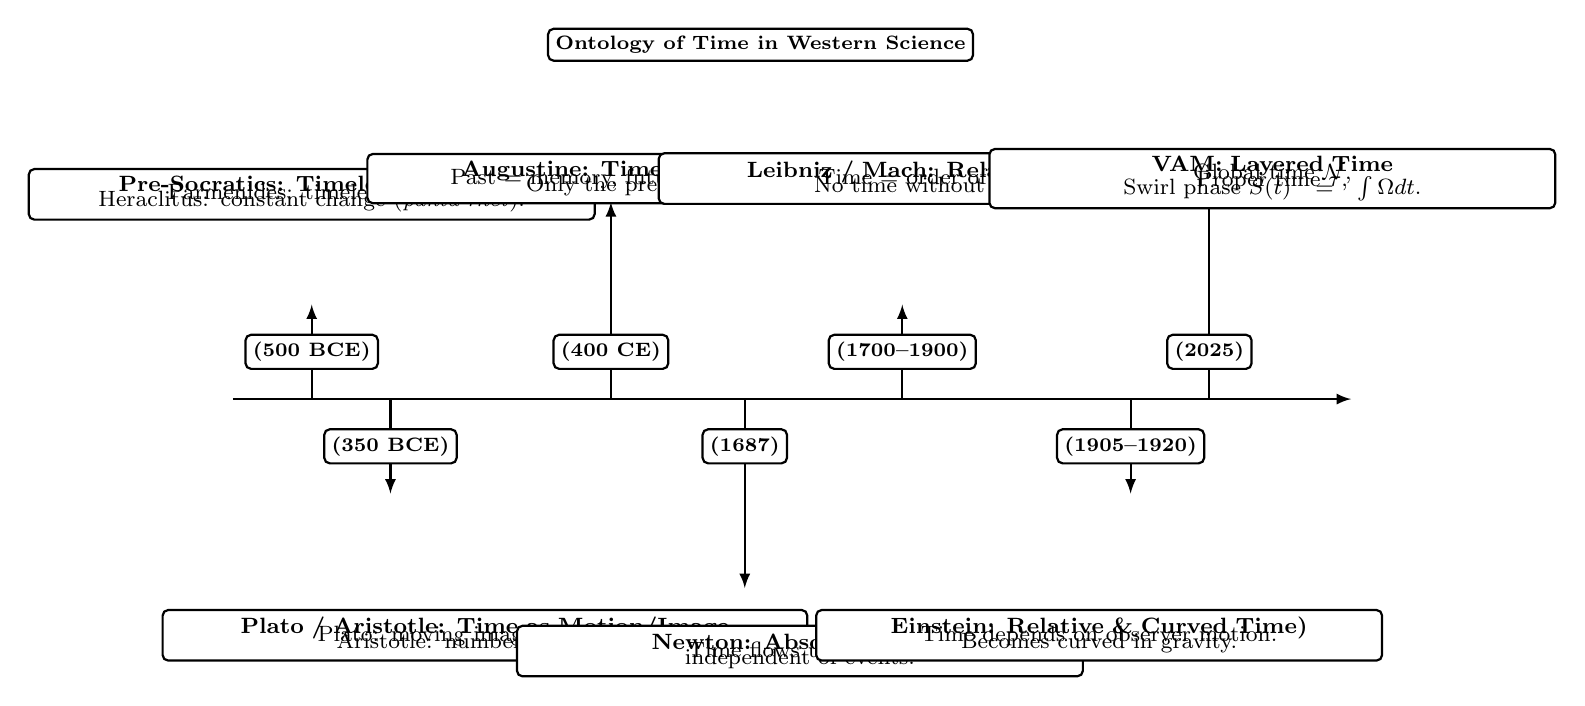
\begin{tikzpicture}[node distance=3.5cm, every node/.style={font=\footnotesize}, >=latex]
\scriptsize


% Timeline base
\draw[->, thick] (-1,0) -- (13.2,0);

% Arrows above timeline (short, as requested)
\draw[->, thick] (0,0) -- (0,1.2);       % Pre-Socratics
\draw[->, thick] (3.8,0) -- (3.8,2.5);   % Augustine
\draw[->, thick] (7.5,0) -- (7.5,1.2);   % Einstein
\draw[->, thick] (11.4,0) -- (11.4,3.0); % VAM

% Arrows below timeline (short, as requested)
\draw[->, thick] (1.0,0) -- (1.0,-1.2);     % Plato/Aristotle
\draw[->, thick] (5.5,0) -- (5.5,-2.4);     % Newton
\draw[->, thick] (10.4,0) -- (10.4,-1.2);     % Leibniz/Mach

    %--- Root title cards (above timeline) ---
\node[draw, thick, rounded corners=2pt, fill=white, align=center, font=\bfseries ] at (0, .6)   {(500 BCE)};
\node[draw, thick, rounded corners=2pt, fill=white, align=center, font=\bfseries ] at (3.8, .6) {(400 CE)};
\node[draw, thick, rounded corners=2pt, fill=white, align=center, font=\bfseries ] at (7.5, .6) {(1700--1900)};
\node[draw, thick, rounded corners=2pt, fill=white, align=center, font=\bfseries ] at (11.4, .6){(2025)};

%--- Root title cards (below timeline) ---
\node[draw, thick, rounded corners=2pt, fill=white, align=center, font=\bfseries ] at (1.0,- .6) {(350 BCE)};
\node[draw, thick, rounded corners=2pt, fill=white, align=center, font=\bfseries ] at (5.5,- .6) {(1687)};
\node[draw, thick, rounded corners=2pt, fill=white, align=center, font=\bfseries ] at (10.4,- .6) {(1905--1920)};

% Label (centered box)
\node[draw, thick, fill=white, rounded corners=2pt, font=\scriptsize] at (5.7,4.5) {\textbf{Ontology of Time in Western Science}};

% Ancient Greek: Parmenides / Heraclitus
\node[draw, rounded corners=2pt, thick, align=center, fill=white, text width=7cm] at (0,2.6) {
\textbf{Pre-Socratics: Timeless vs. Flux}  \\[-0.8em]
Parmenides: timeless being.  \\[-0.8em]
Heraclitus: constant change (\textit{panta rhei}).
};

% Plato / Aristotle
\node[draw, rounded corners=2pt, thick, align=center, fill=white, text width=8cm] at (2.2,-3.0) {
\textbf{Plato / Aristotle: Time as Motion/Image}  \\[-0.8em]
Plato: moving image of eternity.  \\[-0.8em]
Aristotle: number of change.
};

% Augustine
\node[draw, rounded corners=2pt, thick, align=center, fill=white, text width=7cm] at (4.3,2.8) {
\textbf{Augustine: Time as Inner Sense}  \\[-0.8em]
Past = memory, future = anticipation.  \\[-0.8em]
Only the present is real.
};

% Newton
\node[draw, rounded corners=2pt, thick, align=center, fill=white, text width=7cm] at (6.2,-3.2) {
\textbf{Newton: Absolute Time)}  \\[-0.8em]
Time flows uniformly,  \\[-0.8em]
independent of events.
};


% Relationalists: Leibniz / Mach
\node[draw, rounded corners=2pt, thick, align=center, fill=white, text width=7cm] at (8.0,2.8) {
\textbf{Leibniz / Mach: Relational Time}  \\[-0.8em]
Time = order of events.  \\[-0.8em]
No time without change.
};

% Einstein
\node[draw, rounded corners=2pt, thick, align=center, fill=white, text width=7cm] at (10.0,-3.0) {
\textbf{Einstein: Relative \& Curved Time)}  \\[-0.8em]
Time depends on observer motion.  \\[-0.8em]
Becomes curved in gravity.
};


% VAM
\node[draw, rounded corners=2pt, thick, align=center, fill=white, text width=7cm] at (12.2,2.8) {
\textbf{VAM: Layered Time}  \\[-0.8em]
Global time \( \mathcal{N} \),  \\[-0.8em]
Proper time \( \tau \),  \\[-0.8em]
Swirl phase \( S(t) = \int \Omega dt \).
};


\end{tikzpicture}
\captionof{figure}{Historical evolution of temporal ontology: from pre-Socratic polarity to Einstein's spacetime and the layered temporality of the Vortex Æther Model.}
\end{center}
\begin{center}
\footnotesize
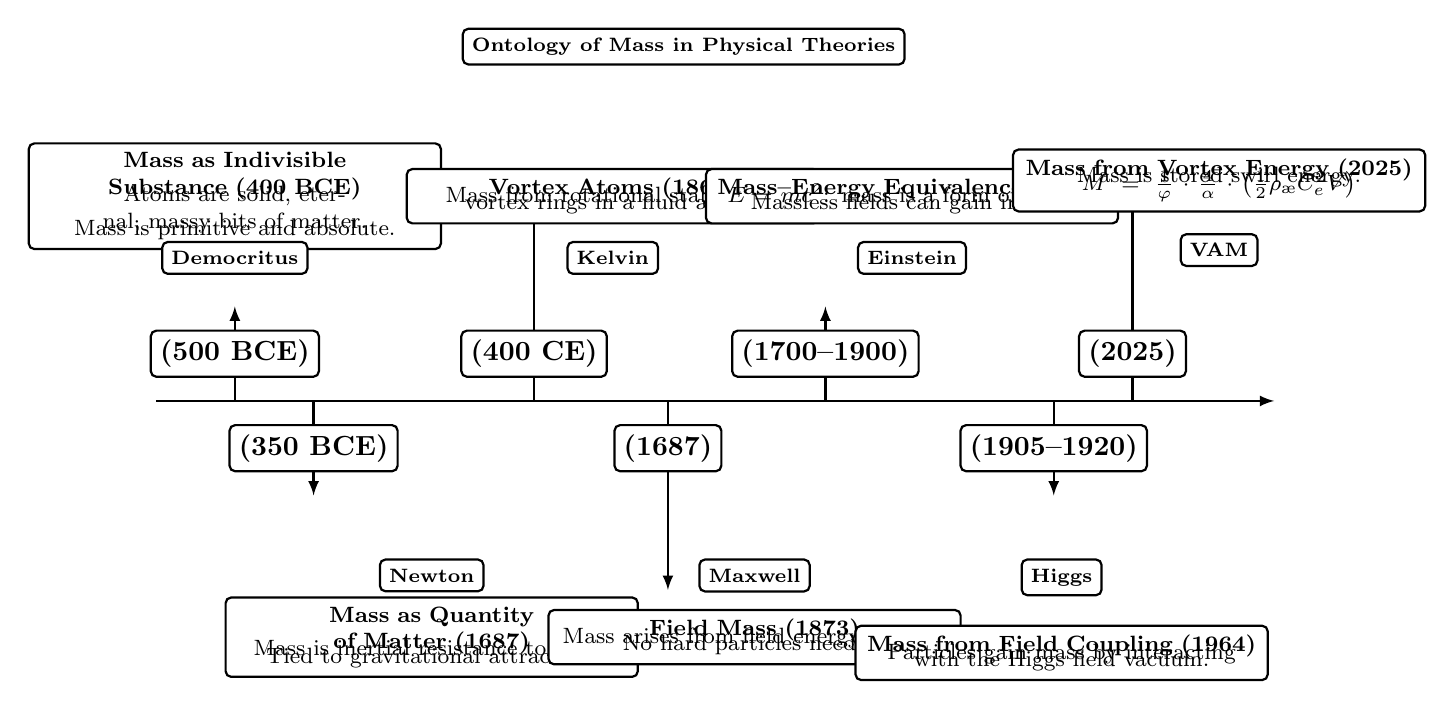
\begin{tikzpicture}[node distance=3.5cm, every node/.style={font=\footnotesize}, >=latex]


% Timeline base
\draw[->, thick] (-1,0) -- (13.2,0);

% Arrows above timeline (short, as requested)
\draw[->, thick] (0,0) -- (0,1.2);       % Pre-Socratics
\draw[->, thick] (3.8,0) -- (3.8,2.5);   % Augustine
\draw[->, thick] (7.5,0) -- (7.5,1.2);   % Einstein
\draw[->, thick] (11.4,0) -- (11.4,3.0); % VAM

% Arrows below timeline (short, as requested)
\draw[->, thick] (1.0,0) -- (1.0,-1.2);     % Plato/Aristotle
\draw[->, thick] (5.5,0) -- (5.5,-2.4);     % Newton
\draw[->, thick] (10.4,0) -- (10.4,-1.2);     % Leibniz/Mach

    %--- Root title cards (above timeline) ---
\node[draw, thick, rounded corners=2pt, fill=white, align=center, font=\bfseries ] at (0, .6)   {(500 BCE)};
\node[draw, thick, rounded corners=2pt, fill=white, align=center, font=\bfseries ] at (3.8, .6) {(400 CE)};
\node[draw, thick, rounded corners=2pt, fill=white, align=center, font=\bfseries ] at (7.5, .6) {(1700--1900)};
\node[draw, thick, rounded corners=2pt, fill=white, align=center, font=\bfseries ] at (11.4, .6){(2025)};

%--- Root title cards (below timeline) ---
\node[draw, thick, rounded corners=2pt, fill=white, align=center, font=\bfseries ] at (1.0,- .6) {(350 BCE)};
\node[draw, thick, rounded corners=2pt, fill=white, align=center, font=\bfseries ] at (5.5,- .6) {(1687)};
\node[draw, thick, rounded corners=2pt, fill=white, align=center, font=\bfseries ] at (10.4,- .6) {(1905--1920)};

% Label
\node[draw, thick, fill=white, rounded corners=2pt, font=\scriptsize] at (5.7,4.5) {\textbf{Ontology of Mass in Physical Theories}};

% Democritus (left)
\node[draw, rounded corners=2pt, thick, align=center, fill=white, text width=5cm] at (0,2.6) {
\textbf{Mass as Indivisible Substance (400 BCE)}  \\[-0.8em]
Atoms are solid, eternal, massy bits of matter.  \\[-0.8em]
Mass is primitive and absolute.
};

\node[above=1.6cm, draw, thick, fill=white, rounded corners=2pt, font=\scriptsize] at (0,0) {\textbf{Democritus}};

% Newton (below)
\node[draw, rounded corners=2pt, thick, align=center, fill=white, text width=5cm] at (2.5,-3.0) {
\textbf{Mass as Quantity of Matter (1687)}  \\[-0.8em]
Mass is inertial resistance to force.  \\[-0.8em]
Tied to gravitational attraction.
};

\node[below=2.0cm, draw, thick, fill=white, rounded corners=2pt, font=\scriptsize] at (2.5,0) {\textbf{Newton}};

% Kelvin (top)
\node[draw, rounded corners=2pt, thick, align=center, fill=white, text width=5cm] at (4.8,2.6) {
\textbf{Vortex Atoms (1867)}  \\[-0.8em]
Mass from rotational stability of  \\[-0.8em]
vortex rings in a fluid æther.
};

\node[above=1.6cm, draw, thick, fill=white, rounded corners=2pt, font=\scriptsize] at (4.8,0) {\textbf{Kelvin}};

% Maxwell (bottom)
\node[draw, rounded corners=2pt, thick, align=center, fill=white, text width=5cm] at (6.6,-3.0) {
\textbf{Field Mass (1873)}  \\[-0.8em]
Mass arises from field energy density.  \\[-0.8em]
No hard particles needed.
};

\node[below=2.0cm, draw, thick, fill=white, rounded corners=2pt, font=\scriptsize] at (6.6,0) {\textbf{Maxwell}};

% Einstein (top)
\node[draw, rounded corners=2pt, thick, align=center, fill=white, text width=5cm] at (8.6,2.6) {
\textbf{Mass–Energy Equivalence (1905)}  \\[-0.8em]
\( E = mc^2 \): mass is a form of energy.  \\[-0.8em]
Massless fields can gain inertia.
};

\node[above=1.6cm, draw, thick, fill=white, rounded corners=2pt, font=\scriptsize] at (8.6,0) {\textbf{Einstein}};

% Higgs (bottom)
\node[draw, rounded corners=2pt, thick, align=center, fill=white, text width=5cm] at (10.5,-3.2) {
\textbf{Mass from Field Coupling (1964)}  \\[-0.8em]
Particles gain mass by interacting  \\[-0.8em]
with the Higgs field vacuum.
};

\node[below=2.0cm, draw, thick, fill=white, rounded corners=2pt, font=\scriptsize] at (10.5,0) {\textbf{Higgs}};

% VAM (top right)
\node[draw, rounded corners=2pt, thick, align=center, fill=white, text width=5cm] at (12.5,2.8) {
\textbf{Mass from Vortex Energy (2025)}  \\[-0.8em]
Mass is stored swirl energy:  \\[-0.8em]
\( M = \frac{1}{\varphi} \cdot \frac{4}{\alpha} \cdot \left( \frac{1}{2} \rho_\text{\ae} C_e^2 V \right) \)
};

\node[above=1.7cm, draw, thick, fill=white, rounded corners=2pt, font=\scriptsize] at (12.5,0) {\textbf{VAM}};

\end{tikzpicture}
\captionof{figure}{Historical evolution of mass ontology: from indivisible substance to field energy and finally to vortex-stored rotational energy in the ætheric continuum of VAM.}
\end{center}

        \section*{Final Reflection: Æther Past and Future}
            These appendices trace a conceptual lineage—beginning with Maxwell's mechanical æther as a carrier of field stresses, evolving through Kelvin's vision of atoms as knotted vortex rings, and reformulated by Einstein into a geometric substrate underlying spacetime itself. Each step preserved the core intuition: that empty space is not truly empty, but possesses structure, energy, and dynamical influence.
            The Vortex Æther Model (VAM) completes this lineage by merging the fluid and field paradigms into a unified topological framework. In VAM, the æther is no longer an abstract scaffolding or discarded relic, but a physically real medium: incompressible, inviscid, and threaded with quantized vorticity. Mass arises from rotational energy; gravity from swirl-induced pressure gradients; time from the internal phase of topological knots.
            Where previous æther models lacked formal consistency or empirical validation, VAM draws on modern tools—fluid dynamics, knot theory, Hamiltonian flows, and high-precision measurement—to revisit the æther hypothesis with scientific rigor and predictive power.
            Einstein redefined the æther without abandoning it. VAM takes the next step—restoring motion, structure, and causality to the medium beneath all physical law.



    \bibliographystyle{unsrt}
    \bibliography{VAM-0-From_Einstein_to_the_Vortex_Fluid_paradigm}
\end{document}